
% Default to the notebook output style

    


% Inherit from the specified cell style.




    
\documentclass[11pt]{article}

    
    
    \usepackage[T1]{fontenc}
    % Nicer default font (+ math font) than Computer Modern for most use cases
    \usepackage{mathpazo}

    % Basic figure setup, for now with no caption control since it's done
    % automatically by Pandoc (which extracts ![](path) syntax from Markdown).
    \usepackage{graphicx}
    % We will generate all images so they have a width \maxwidth. This means
    % that they will get their normal width if they fit onto the page, but
    % are scaled down if they would overflow the margins.
    \makeatletter
    \def\maxwidth{\ifdim\Gin@nat@width>\linewidth\linewidth
    \else\Gin@nat@width\fi}
    \makeatother
    \let\Oldincludegraphics\includegraphics
    % Set max figure width to be 80% of text width, for now hardcoded.
    \renewcommand{\includegraphics}[1]{\Oldincludegraphics[width=.8\maxwidth]{#1}}
    % Ensure that by default, figures have no caption (until we provide a
    % proper Figure object with a Caption API and a way to capture that
    % in the conversion process - todo).
    \usepackage{caption}
    \DeclareCaptionLabelFormat{nolabel}{}
    \captionsetup{labelformat=nolabel}

    \usepackage{adjustbox} % Used to constrain images to a maximum size 
    \usepackage{xcolor} % Allow colors to be defined
    \usepackage{enumerate} % Needed for markdown enumerations to work
    \usepackage{geometry} % Used to adjust the document margins
    \usepackage{amsmath} % Equations
    \usepackage{amssymb} % Equations
    \usepackage{textcomp} % defines textquotesingle
    % Hack from http://tex.stackexchange.com/a/47451/13684:
    \AtBeginDocument{%
        \def\PYZsq{\textquotesingle}% Upright quotes in Pygmentized code
    }
    \usepackage{upquote} % Upright quotes for verbatim code
    \usepackage{eurosym} % defines \euro
    \usepackage[mathletters]{ucs} % Extended unicode (utf-8) support
    \usepackage[utf8x]{inputenc} % Allow utf-8 characters in the tex document
    \usepackage{fancyvrb} % verbatim replacement that allows latex
    \usepackage{grffile} % extends the file name processing of package graphics 
                         % to support a larger range 
    % The hyperref package gives us a pdf with properly built
    % internal navigation ('pdf bookmarks' for the table of contents,
    % internal cross-reference links, web links for URLs, etc.)
    \usepackage{hyperref}
    \usepackage{longtable} % longtable support required by pandoc >1.10
    \usepackage{booktabs}  % table support for pandoc > 1.12.2
    \usepackage[inline]{enumitem} % IRkernel/repr support (it uses the enumerate* environment)
    \usepackage[normalem]{ulem} % ulem is needed to support strikethroughs (\sout)
                                % normalem makes italics be italics, not underlines
    

    
    
    % Colors for the hyperref package
    \definecolor{urlcolor}{rgb}{0,.145,.698}
    \definecolor{linkcolor}{rgb}{.71,0.21,0.01}
    \definecolor{citecolor}{rgb}{.12,.54,.11}

    % ANSI colors
    \definecolor{ansi-black}{HTML}{3E424D}
    \definecolor{ansi-black-intense}{HTML}{282C36}
    \definecolor{ansi-red}{HTML}{E75C58}
    \definecolor{ansi-red-intense}{HTML}{B22B31}
    \definecolor{ansi-green}{HTML}{00A250}
    \definecolor{ansi-green-intense}{HTML}{007427}
    \definecolor{ansi-yellow}{HTML}{DDB62B}
    \definecolor{ansi-yellow-intense}{HTML}{B27D12}
    \definecolor{ansi-blue}{HTML}{208FFB}
    \definecolor{ansi-blue-intense}{HTML}{0065CA}
    \definecolor{ansi-magenta}{HTML}{D160C4}
    \definecolor{ansi-magenta-intense}{HTML}{A03196}
    \definecolor{ansi-cyan}{HTML}{60C6C8}
    \definecolor{ansi-cyan-intense}{HTML}{258F8F}
    \definecolor{ansi-white}{HTML}{C5C1B4}
    \definecolor{ansi-white-intense}{HTML}{A1A6B2}

    % commands and environments needed by pandoc snippets
    % extracted from the output of `pandoc -s`
    \providecommand{\tightlist}{%
      \setlength{\itemsep}{0pt}\setlength{\parskip}{0pt}}
    \DefineVerbatimEnvironment{Highlighting}{Verbatim}{commandchars=\\\{\}}
    % Add ',fontsize=\small' for more characters per line
    \newenvironment{Shaded}{}{}
    \newcommand{\KeywordTok}[1]{\textcolor[rgb]{0.00,0.44,0.13}{\textbf{{#1}}}}
    \newcommand{\DataTypeTok}[1]{\textcolor[rgb]{0.56,0.13,0.00}{{#1}}}
    \newcommand{\DecValTok}[1]{\textcolor[rgb]{0.25,0.63,0.44}{{#1}}}
    \newcommand{\BaseNTok}[1]{\textcolor[rgb]{0.25,0.63,0.44}{{#1}}}
    \newcommand{\FloatTok}[1]{\textcolor[rgb]{0.25,0.63,0.44}{{#1}}}
    \newcommand{\CharTok}[1]{\textcolor[rgb]{0.25,0.44,0.63}{{#1}}}
    \newcommand{\StringTok}[1]{\textcolor[rgb]{0.25,0.44,0.63}{{#1}}}
    \newcommand{\CommentTok}[1]{\textcolor[rgb]{0.38,0.63,0.69}{\textit{{#1}}}}
    \newcommand{\OtherTok}[1]{\textcolor[rgb]{0.00,0.44,0.13}{{#1}}}
    \newcommand{\AlertTok}[1]{\textcolor[rgb]{1.00,0.00,0.00}{\textbf{{#1}}}}
    \newcommand{\FunctionTok}[1]{\textcolor[rgb]{0.02,0.16,0.49}{{#1}}}
    \newcommand{\RegionMarkerTok}[1]{{#1}}
    \newcommand{\ErrorTok}[1]{\textcolor[rgb]{1.00,0.00,0.00}{\textbf{{#1}}}}
    \newcommand{\NormalTok}[1]{{#1}}
    
    % Additional commands for more recent versions of Pandoc
    \newcommand{\ConstantTok}[1]{\textcolor[rgb]{0.53,0.00,0.00}{{#1}}}
    \newcommand{\SpecialCharTok}[1]{\textcolor[rgb]{0.25,0.44,0.63}{{#1}}}
    \newcommand{\VerbatimStringTok}[1]{\textcolor[rgb]{0.25,0.44,0.63}{{#1}}}
    \newcommand{\SpecialStringTok}[1]{\textcolor[rgb]{0.73,0.40,0.53}{{#1}}}
    \newcommand{\ImportTok}[1]{{#1}}
    \newcommand{\DocumentationTok}[1]{\textcolor[rgb]{0.73,0.13,0.13}{\textit{{#1}}}}
    \newcommand{\AnnotationTok}[1]{\textcolor[rgb]{0.38,0.63,0.69}{\textbf{\textit{{#1}}}}}
    \newcommand{\CommentVarTok}[1]{\textcolor[rgb]{0.38,0.63,0.69}{\textbf{\textit{{#1}}}}}
    \newcommand{\VariableTok}[1]{\textcolor[rgb]{0.10,0.09,0.49}{{#1}}}
    \newcommand{\ControlFlowTok}[1]{\textcolor[rgb]{0.00,0.44,0.13}{\textbf{{#1}}}}
    \newcommand{\OperatorTok}[1]{\textcolor[rgb]{0.40,0.40,0.40}{{#1}}}
    \newcommand{\BuiltInTok}[1]{{#1}}
    \newcommand{\ExtensionTok}[1]{{#1}}
    \newcommand{\PreprocessorTok}[1]{\textcolor[rgb]{0.74,0.48,0.00}{{#1}}}
    \newcommand{\AttributeTok}[1]{\textcolor[rgb]{0.49,0.56,0.16}{{#1}}}
    \newcommand{\InformationTok}[1]{\textcolor[rgb]{0.38,0.63,0.69}{\textbf{\textit{{#1}}}}}
    \newcommand{\WarningTok}[1]{\textcolor[rgb]{0.38,0.63,0.69}{\textbf{\textit{{#1}}}}}
    
    
    % Define a nice break command that doesn't care if a line doesn't already
    % exist.
    \def\br{\hspace*{\fill} \\* }
    % Math Jax compatability definitions
    \def\gt{>}
    \def\lt{<}
    % Document parameters
    \title{dbGaP2x}
    
    
    

    % Pygments definitions
    
\makeatletter
\def\PY@reset{\let\PY@it=\relax \let\PY@bf=\relax%
    \let\PY@ul=\relax \let\PY@tc=\relax%
    \let\PY@bc=\relax \let\PY@ff=\relax}
\def\PY@tok#1{\csname PY@tok@#1\endcsname}
\def\PY@toks#1+{\ifx\relax#1\empty\else%
    \PY@tok{#1}\expandafter\PY@toks\fi}
\def\PY@do#1{\PY@bc{\PY@tc{\PY@ul{%
    \PY@it{\PY@bf{\PY@ff{#1}}}}}}}
\def\PY#1#2{\PY@reset\PY@toks#1+\relax+\PY@do{#2}}

\expandafter\def\csname PY@tok@w\endcsname{\def\PY@tc##1{\textcolor[rgb]{0.73,0.73,0.73}{##1}}}
\expandafter\def\csname PY@tok@c\endcsname{\let\PY@it=\textit\def\PY@tc##1{\textcolor[rgb]{0.25,0.50,0.50}{##1}}}
\expandafter\def\csname PY@tok@cp\endcsname{\def\PY@tc##1{\textcolor[rgb]{0.74,0.48,0.00}{##1}}}
\expandafter\def\csname PY@tok@k\endcsname{\let\PY@bf=\textbf\def\PY@tc##1{\textcolor[rgb]{0.00,0.50,0.00}{##1}}}
\expandafter\def\csname PY@tok@kp\endcsname{\def\PY@tc##1{\textcolor[rgb]{0.00,0.50,0.00}{##1}}}
\expandafter\def\csname PY@tok@kt\endcsname{\def\PY@tc##1{\textcolor[rgb]{0.69,0.00,0.25}{##1}}}
\expandafter\def\csname PY@tok@o\endcsname{\def\PY@tc##1{\textcolor[rgb]{0.40,0.40,0.40}{##1}}}
\expandafter\def\csname PY@tok@ow\endcsname{\let\PY@bf=\textbf\def\PY@tc##1{\textcolor[rgb]{0.67,0.13,1.00}{##1}}}
\expandafter\def\csname PY@tok@nb\endcsname{\def\PY@tc##1{\textcolor[rgb]{0.00,0.50,0.00}{##1}}}
\expandafter\def\csname PY@tok@nf\endcsname{\def\PY@tc##1{\textcolor[rgb]{0.00,0.00,1.00}{##1}}}
\expandafter\def\csname PY@tok@nc\endcsname{\let\PY@bf=\textbf\def\PY@tc##1{\textcolor[rgb]{0.00,0.00,1.00}{##1}}}
\expandafter\def\csname PY@tok@nn\endcsname{\let\PY@bf=\textbf\def\PY@tc##1{\textcolor[rgb]{0.00,0.00,1.00}{##1}}}
\expandafter\def\csname PY@tok@ne\endcsname{\let\PY@bf=\textbf\def\PY@tc##1{\textcolor[rgb]{0.82,0.25,0.23}{##1}}}
\expandafter\def\csname PY@tok@nv\endcsname{\def\PY@tc##1{\textcolor[rgb]{0.10,0.09,0.49}{##1}}}
\expandafter\def\csname PY@tok@no\endcsname{\def\PY@tc##1{\textcolor[rgb]{0.53,0.00,0.00}{##1}}}
\expandafter\def\csname PY@tok@nl\endcsname{\def\PY@tc##1{\textcolor[rgb]{0.63,0.63,0.00}{##1}}}
\expandafter\def\csname PY@tok@ni\endcsname{\let\PY@bf=\textbf\def\PY@tc##1{\textcolor[rgb]{0.60,0.60,0.60}{##1}}}
\expandafter\def\csname PY@tok@na\endcsname{\def\PY@tc##1{\textcolor[rgb]{0.49,0.56,0.16}{##1}}}
\expandafter\def\csname PY@tok@nt\endcsname{\let\PY@bf=\textbf\def\PY@tc##1{\textcolor[rgb]{0.00,0.50,0.00}{##1}}}
\expandafter\def\csname PY@tok@nd\endcsname{\def\PY@tc##1{\textcolor[rgb]{0.67,0.13,1.00}{##1}}}
\expandafter\def\csname PY@tok@s\endcsname{\def\PY@tc##1{\textcolor[rgb]{0.73,0.13,0.13}{##1}}}
\expandafter\def\csname PY@tok@sd\endcsname{\let\PY@it=\textit\def\PY@tc##1{\textcolor[rgb]{0.73,0.13,0.13}{##1}}}
\expandafter\def\csname PY@tok@si\endcsname{\let\PY@bf=\textbf\def\PY@tc##1{\textcolor[rgb]{0.73,0.40,0.53}{##1}}}
\expandafter\def\csname PY@tok@se\endcsname{\let\PY@bf=\textbf\def\PY@tc##1{\textcolor[rgb]{0.73,0.40,0.13}{##1}}}
\expandafter\def\csname PY@tok@sr\endcsname{\def\PY@tc##1{\textcolor[rgb]{0.73,0.40,0.53}{##1}}}
\expandafter\def\csname PY@tok@ss\endcsname{\def\PY@tc##1{\textcolor[rgb]{0.10,0.09,0.49}{##1}}}
\expandafter\def\csname PY@tok@sx\endcsname{\def\PY@tc##1{\textcolor[rgb]{0.00,0.50,0.00}{##1}}}
\expandafter\def\csname PY@tok@m\endcsname{\def\PY@tc##1{\textcolor[rgb]{0.40,0.40,0.40}{##1}}}
\expandafter\def\csname PY@tok@gh\endcsname{\let\PY@bf=\textbf\def\PY@tc##1{\textcolor[rgb]{0.00,0.00,0.50}{##1}}}
\expandafter\def\csname PY@tok@gu\endcsname{\let\PY@bf=\textbf\def\PY@tc##1{\textcolor[rgb]{0.50,0.00,0.50}{##1}}}
\expandafter\def\csname PY@tok@gd\endcsname{\def\PY@tc##1{\textcolor[rgb]{0.63,0.00,0.00}{##1}}}
\expandafter\def\csname PY@tok@gi\endcsname{\def\PY@tc##1{\textcolor[rgb]{0.00,0.63,0.00}{##1}}}
\expandafter\def\csname PY@tok@gr\endcsname{\def\PY@tc##1{\textcolor[rgb]{1.00,0.00,0.00}{##1}}}
\expandafter\def\csname PY@tok@ge\endcsname{\let\PY@it=\textit}
\expandafter\def\csname PY@tok@gs\endcsname{\let\PY@bf=\textbf}
\expandafter\def\csname PY@tok@gp\endcsname{\let\PY@bf=\textbf\def\PY@tc##1{\textcolor[rgb]{0.00,0.00,0.50}{##1}}}
\expandafter\def\csname PY@tok@go\endcsname{\def\PY@tc##1{\textcolor[rgb]{0.53,0.53,0.53}{##1}}}
\expandafter\def\csname PY@tok@gt\endcsname{\def\PY@tc##1{\textcolor[rgb]{0.00,0.27,0.87}{##1}}}
\expandafter\def\csname PY@tok@err\endcsname{\def\PY@bc##1{\setlength{\fboxsep}{0pt}\fcolorbox[rgb]{1.00,0.00,0.00}{1,1,1}{\strut ##1}}}
\expandafter\def\csname PY@tok@kc\endcsname{\let\PY@bf=\textbf\def\PY@tc##1{\textcolor[rgb]{0.00,0.50,0.00}{##1}}}
\expandafter\def\csname PY@tok@kd\endcsname{\let\PY@bf=\textbf\def\PY@tc##1{\textcolor[rgb]{0.00,0.50,0.00}{##1}}}
\expandafter\def\csname PY@tok@kn\endcsname{\let\PY@bf=\textbf\def\PY@tc##1{\textcolor[rgb]{0.00,0.50,0.00}{##1}}}
\expandafter\def\csname PY@tok@kr\endcsname{\let\PY@bf=\textbf\def\PY@tc##1{\textcolor[rgb]{0.00,0.50,0.00}{##1}}}
\expandafter\def\csname PY@tok@bp\endcsname{\def\PY@tc##1{\textcolor[rgb]{0.00,0.50,0.00}{##1}}}
\expandafter\def\csname PY@tok@fm\endcsname{\def\PY@tc##1{\textcolor[rgb]{0.00,0.00,1.00}{##1}}}
\expandafter\def\csname PY@tok@vc\endcsname{\def\PY@tc##1{\textcolor[rgb]{0.10,0.09,0.49}{##1}}}
\expandafter\def\csname PY@tok@vg\endcsname{\def\PY@tc##1{\textcolor[rgb]{0.10,0.09,0.49}{##1}}}
\expandafter\def\csname PY@tok@vi\endcsname{\def\PY@tc##1{\textcolor[rgb]{0.10,0.09,0.49}{##1}}}
\expandafter\def\csname PY@tok@vm\endcsname{\def\PY@tc##1{\textcolor[rgb]{0.10,0.09,0.49}{##1}}}
\expandafter\def\csname PY@tok@sa\endcsname{\def\PY@tc##1{\textcolor[rgb]{0.73,0.13,0.13}{##1}}}
\expandafter\def\csname PY@tok@sb\endcsname{\def\PY@tc##1{\textcolor[rgb]{0.73,0.13,0.13}{##1}}}
\expandafter\def\csname PY@tok@sc\endcsname{\def\PY@tc##1{\textcolor[rgb]{0.73,0.13,0.13}{##1}}}
\expandafter\def\csname PY@tok@dl\endcsname{\def\PY@tc##1{\textcolor[rgb]{0.73,0.13,0.13}{##1}}}
\expandafter\def\csname PY@tok@s2\endcsname{\def\PY@tc##1{\textcolor[rgb]{0.73,0.13,0.13}{##1}}}
\expandafter\def\csname PY@tok@sh\endcsname{\def\PY@tc##1{\textcolor[rgb]{0.73,0.13,0.13}{##1}}}
\expandafter\def\csname PY@tok@s1\endcsname{\def\PY@tc##1{\textcolor[rgb]{0.73,0.13,0.13}{##1}}}
\expandafter\def\csname PY@tok@mb\endcsname{\def\PY@tc##1{\textcolor[rgb]{0.40,0.40,0.40}{##1}}}
\expandafter\def\csname PY@tok@mf\endcsname{\def\PY@tc##1{\textcolor[rgb]{0.40,0.40,0.40}{##1}}}
\expandafter\def\csname PY@tok@mh\endcsname{\def\PY@tc##1{\textcolor[rgb]{0.40,0.40,0.40}{##1}}}
\expandafter\def\csname PY@tok@mi\endcsname{\def\PY@tc##1{\textcolor[rgb]{0.40,0.40,0.40}{##1}}}
\expandafter\def\csname PY@tok@il\endcsname{\def\PY@tc##1{\textcolor[rgb]{0.40,0.40,0.40}{##1}}}
\expandafter\def\csname PY@tok@mo\endcsname{\def\PY@tc##1{\textcolor[rgb]{0.40,0.40,0.40}{##1}}}
\expandafter\def\csname PY@tok@ch\endcsname{\let\PY@it=\textit\def\PY@tc##1{\textcolor[rgb]{0.25,0.50,0.50}{##1}}}
\expandafter\def\csname PY@tok@cm\endcsname{\let\PY@it=\textit\def\PY@tc##1{\textcolor[rgb]{0.25,0.50,0.50}{##1}}}
\expandafter\def\csname PY@tok@cpf\endcsname{\let\PY@it=\textit\def\PY@tc##1{\textcolor[rgb]{0.25,0.50,0.50}{##1}}}
\expandafter\def\csname PY@tok@c1\endcsname{\let\PY@it=\textit\def\PY@tc##1{\textcolor[rgb]{0.25,0.50,0.50}{##1}}}
\expandafter\def\csname PY@tok@cs\endcsname{\let\PY@it=\textit\def\PY@tc##1{\textcolor[rgb]{0.25,0.50,0.50}{##1}}}

\def\PYZbs{\char`\\}
\def\PYZus{\char`\_}
\def\PYZob{\char`\{}
\def\PYZcb{\char`\}}
\def\PYZca{\char`\^}
\def\PYZam{\char`\&}
\def\PYZlt{\char`\<}
\def\PYZgt{\char`\>}
\def\PYZsh{\char`\#}
\def\PYZpc{\char`\%}
\def\PYZdl{\char`\$}
\def\PYZhy{\char`\-}
\def\PYZsq{\char`\'}
\def\PYZdq{\char`\"}
\def\PYZti{\char`\~}
% for compatibility with earlier versions
\def\PYZat{@}
\def\PYZlb{[}
\def\PYZrb{]}
\makeatother


    % Exact colors from NB
    \definecolor{incolor}{rgb}{0.0, 0.0, 0.5}
    \definecolor{outcolor}{rgb}{0.545, 0.0, 0.0}



    
    % Prevent overflowing lines due to hard-to-break entities
    \sloppy 
    % Setup hyperref package
    \hypersetup{
      breaklinks=true,  % so long urls are correctly broken across lines
      colorlinks=true,
      urlcolor=urlcolor,
      linkcolor=linkcolor,
      citecolor=citecolor,
      }
    % Slightly bigger margins than the latex defaults
    
    \geometry{verbose,tmargin=1in,bmargin=1in,lmargin=1in,rmargin=1in}
    
    

    \begin{document}
    
    
    \maketitle
    
    

    
    \hypertarget{using-dbgap2x-r-package-to-explore-and-sort-phenotypics-data-from-dbgap}{%
\section{Using dbGaP2x, R package to explore and sort phenotypics data
from
dbGap}\label{using-dbgap2x-r-package-to-explore-and-sort-phenotypics-data-from-dbgap}}

    \hypertarget{introduction}{%
\subsection{Introduction}\label{introduction}}

\hypertarget{load-the-package}{%
\subsubsection{Load the package}\label{load-the-package}}

    \begin{Verbatim}[commandchars=\\\{\}]
{\color{incolor}In [{\color{incolor}1}]:} \PY{c+c1}{\PYZsh{}devtools::install\PYZus{}github(\PYZdq{}gversmee/dbGaP2x\PYZdq{}, force = TRUE)}
        \PY{k+kn}{library}\PY{p}{(}dbGaP2x\PY{p}{)}
\end{Verbatim}


    \hypertarget{get-the-list-of-the-function-for-this-new-package}{%
\subsubsection{Get the list of the function for this new
package}\label{get-the-list-of-the-function-for-this-new-package}}

    \begin{Verbatim}[commandchars=\\\{\}]
{\color{incolor}In [{\color{incolor}2}]:} lsf.str\PY{p}{(}\PY{l+s}{\PYZdq{}}\PY{l+s}{package:dbGaP2x\PYZdq{}}\PY{p}{)}
\end{Verbatim}


    
    \begin{verbatim}
browse.dbgap : function (phs, jupyter = FALSE)  
browse.study : function (phs, jupyter = FALSE)  
consent.groups : function (phs)  
datatables.dict : function (phs)  
dbgap.data_dict : function (xml, dest)  
dbgap.decrypt : function (files, key = FALSE)  
dbgap.download : function (krt, key = FALSE)  
is.parent : function (phs)  
n.pop : function (phs, consentgroups = TRUE, gender = TRUE)  
n.tables : function (phs)  
n.variables : function (phs)  
parent.study : function (phs)  
phs.version : function (phs)  
search.dbgap : function (term, jupyter = FALSE)  
study.name : function (phs)  
sub.study : function (phs)  
variables.dict : function (phs)  
    \end{verbatim}

    
    \hypertarget{search-for-dbgap-studies}{%
\subsection{Search for dbGap studies}\label{search-for-dbgap-studies}}

\hypertarget{lets-try-to-explore-the-jackson-heart-study-cohort-that-exists-on-dbgap.}{%
\subsubsection{Let's try to explore the ``Jackson Heart Study'' cohort
that exists on
dbGap.}\label{lets-try-to-explore-the-jackson-heart-study-cohort-that-exists-on-dbgap.}}

The dbGap search engine can be tricky, that's why we created the
function ``browse.dbgap'', who helps you find the studies related to the
term that you search on your web browser.

Note that if you run this function in a jupyterhub environment, it will
return a url since jupyterhub doesn't have access to your local browser.

    \begin{Verbatim}[commandchars=\\\{\}]
{\color{incolor}In [{\color{incolor}3}]:} search.dbgap\PY{p}{(}\PY{l+s}{\PYZdq{}}\PY{l+s}{Jackson\PYZdq{}}\PY{p}{,} jupyter \PY{o}{=} \PY{k+kc}{TRUE}\PY{p}{)}
\end{Verbatim}


    'https://www.ncbi.nlm.nih.gov/gap/?term=Jackson\%5BStudy+Name\%5D'

    
    \hypertarget{dbgap-returns-the-list-of-the-studies-related-to-your-term.-as-you-see-there-are-6-studies-associated-with-the-jackson-heart-study-jhs.-one-of-these-study-is-the-main-one-aka-the-parent-study-whereas-the-other-ones-are-substudies.-in-this-case-phs000286.v5.p1-is-the-parent-study.-firslty-we-can-use-the-phs.version-function-in-order-to-be-sure-that-this-is-the-latest-version-of-the-study.-we-can-abbreviate-the-phs-name-by-giving-just-the-digit-or-we-can-use-the-full-dbgap-id.}{%
\paragraph{dbGap returns the list of the studies related to your term.
As you see, there are 6 studies associated with the ``Jackson Heart
Study'' (JHS). One of these study is the main one aka the ``parent
study'', whereas the other ones are substudies. In this case,
phs000286.v5.p1 is the parent study. Firslty, we can use the
phs.version() function in order to be sure that this is the latest
version of the study. We can abbreviate the phs name by giving just the
digit, or we can use the full dbGap
id.}\label{dbgap-returns-the-list-of-the-studies-related-to-your-term.-as-you-see-there-are-6-studies-associated-with-the-jackson-heart-study-jhs.-one-of-these-study-is-the-main-one-aka-the-parent-study-whereas-the-other-ones-are-substudies.-in-this-case-phs000286.v5.p1-is-the-parent-study.-firslty-we-can-use-the-phs.version-function-in-order-to-be-sure-that-this-is-the-latest-version-of-the-study.-we-can-abbreviate-the-phs-name-by-giving-just-the-digit-or-we-can-use-the-full-dbgap-id.}}

    \begin{Verbatim}[commandchars=\\\{\}]
{\color{incolor}In [{\color{incolor}4}]:} phs.version\PY{p}{(}\PY{l+s}{\PYZdq{}}\PY{l+s}{286\PYZdq{}}\PY{p}{)}
\end{Verbatim}


    'phs000286.v5.p1'

    
    \hypertarget{the-is.parent-function-is-usefull-to-test-if-a-study-is-a-parent-study-or-a-substudy}{%
\subparagraph{The is.parent() function is usefull to test if a study is
a parent study or a
substudy}\label{the-is.parent-function-is-usefull-to-test-if-a-study-is-a-parent-study-or-a-substudy}}

    \begin{Verbatim}[commandchars=\\\{\}]
{\color{incolor}In [{\color{incolor}5}]:} is.parent\PY{p}{(}\PY{l+s}{\PYZdq{}}\PY{l+s}{000286\PYZdq{}}\PY{p}{)} \PY{c+c1}{\PYZsh{} JHS main cohort}
        is.parent\PY{p}{(}\PY{l+s}{\PYZdq{}}\PY{l+s}{phs499\PYZdq{}}\PY{p}{)} \PY{c+c1}{\PYZsh{} substudy \PYZdq{}CARe\PYZdq{} for JHS}
\end{Verbatim}


    TRUE

    
    FALSE

    
    \hypertarget{if-you-dont-know-the-parent-study-of-a-substudy-try-parent.study}{%
\paragraph{If you don't know the parent study of a substudy, try
parent.study()}\label{if-you-dont-know-the-parent-study-of-a-substudy-try-parent.study}}

    \begin{Verbatim}[commandchars=\\\{\}]
{\color{incolor}In [{\color{incolor}6}]:} parent.study\PY{p}{(}\PY{l+s}{\PYZdq{}}\PY{l+s}{phs000499\PYZdq{}}\PY{p}{)}
\end{Verbatim}


    \begin{enumerate*}
\item 'phs000286.v5.p1'
\item 'Jackson Heart Study (JHS) Cohort'
\end{enumerate*}


    
    \hypertarget{on-the-other-side-use-sub.study-to-get-the-name-and-ids-of-the-substudies-from-a-parent-one}{%
\subparagraph{On the other side, use sub.study() to get the name and IDs
of the substudies from a parent
one}\label{on-the-other-side-use-sub.study-to-get-the-name-and-ids-of-the-substudies-from-a-parent-one}}

    \begin{Verbatim}[commandchars=\\\{\}]
{\color{incolor}In [{\color{incolor}7}]:} sub.study\PY{p}{(}\PY{l+s}{\PYZdq{}}\PY{l+s}{286\PYZdq{}}\PY{p}{)}
\end{Verbatim}


    \begin{tabular}{ll}
 phs & name\\
\hline
	 phs000499.v3.p1                                                      & NHLBI Jackson Heart Study Candidate Gene Association Resource (CARe)\\
	 phs000498.v3.p1                                                      & Jackson Heart Study Allelic Spectrum Project                        \\
	 phs000402.v3.p1                                                      & NHLBI GO-ESP: Heart Cohorts Exome Sequencing Project (JHS)          \\
	 phs001098.v1.p1                                                      & T2D-GENES Multi-Ethnic Exome Sequencing Study: Jackson Heart Study  \\
\end{tabular}


    
    \hypertarget{if-you-want-to-get-the-name-of-a-study-from-its-dbgap-id-use-study.name}{%
\subparagraph{If you want to get the name of a study from its dbGap id,
use
study.name()}\label{if-you-want-to-get-the-name-of-a-study-from-its-dbgap-id-use-study.name}}

    \begin{Verbatim}[commandchars=\\\{\}]
{\color{incolor}In [{\color{incolor}8}]:} study.name\PY{p}{(}\PY{l+s}{\PYZdq{}}\PY{l+s}{286\PYZdq{}}\PY{p}{)}
\end{Verbatim}


    'Jackson Heart Study (JHS) Cohort'

    
    \hypertarget{finally-you-can-watch-your-study-on-dbgap-with-browse.dbgap.}{%
\subparagraph{Finally, you can watch your study on dbGap with
browse.dbgap().}\label{finally-you-can-watch-your-study-on-dbgap-with-browse.dbgap.}}

\hypertarget{if-a-website-exists-for-this-study-you-can-browse-it-using-browse.study}{%
\subparagraph{If a website exists for this study, you can browse it
using
browse.study()}\label{if-a-website-exists-for-this-study-you-can-browse-it-using-browse.study}}

    \begin{Verbatim}[commandchars=\\\{\}]
{\color{incolor}In [{\color{incolor}9}]:} browse.dbgap\PY{p}{(}\PY{l+s}{\PYZdq{}}\PY{l+s}{286\PYZdq{}}\PY{p}{,} jupyter \PY{o}{=} \PY{k+kc}{TRUE}\PY{p}{)}
        browse.study\PY{p}{(}\PY{l+s}{\PYZdq{}}\PY{l+s}{286\PYZdq{}}\PY{p}{,} jupyter \PY{o}{=} \PY{k+kc}{TRUE}\PY{p}{)}
\end{Verbatim}


    'https://www.ncbi.nlm.nih.gov/projects/gap/cgi-bin/study.cgi?study\_id=phs000286.v5.p1'

    
    'https://www.jacksonheartstudy.org'

    
    \hypertarget{explore-the-characteristics-of-your-study}{%
\subsection{Explore the characteristics of your
study}\label{explore-the-characteristics-of-your-study}}

\hypertarget{for-each-dbgap-study-there-can-be-multiple-consent-groups-that-will-have-there-specificities.-use-consent.groups-to-know-the-number-and-the-name-of-the-consent-groups-in-the-study-that-you-are-exploring.-lets-keep-focusing-on-jhs.}{%
\subparagraph{For each dbGap study, there can be multiple consent groups
that will have there specificities. Use consent.groups to know the
number and the name of the consent groups in the study that you are
exploring. Let's keep focusing on
JHS.}\label{for-each-dbgap-study-there-can-be-multiple-consent-groups-that-will-have-there-specificities.-use-consent.groups-to-know-the-number-and-the-name-of-the-consent-groups-in-the-study-that-you-are-exploring.-lets-keep-focusing-on-jhs.}}

    \begin{Verbatim}[commandchars=\\\{\}]
{\color{incolor}In [{\color{incolor}10}]:} JHS \PY{o}{\PYZlt{}\PYZhy{}} \PY{l+s}{\PYZdq{}}\PY{l+s}{phs000286\PYZdq{}}
         consent.groups\PY{p}{(}JHS\PY{p}{)}
\end{Verbatim}


    \begin{tabular}{r|ll}
  & shortName & longName\\
\hline
	0 & NRUP                                                                                                                                                                              & Subjects did not participate in the study, did not complete a consent document and are included only for the pedigree structure and/or genotype controls, such as HapMap subjects\\
	1 & HMB-IRB-NPU                                                                                                                                                                       & Health/Medical/Biomedical (IRB, NPU)                                                                                                                                             \\
	2 & DS-FDO-IRB-NPU                                                                                                                                                                    & Disease-Specific (Focused Disease Only, IRB, NPU)                                                                                                                                \\
	3 & HMB-IRB                                                                                                                                                                           & Health/Medical/Biomedical (IRB)                                                                                                                                                  \\
	4 & DS-FDO-IRB                                                                                                                                                                        & Disease-Specific (Focused Disease Only, IRB)                                                                                                                                     \\
\end{tabular}


    
    \hypertarget{use-n.pop-to-know-the-number-of-patient-included-in-each-groups}{%
\subparagraph{Use n.pop() to know the number of patient included in each
groups}\label{use-n.pop-to-know-the-number-of-patient-included-in-each-groups}}

    \begin{Verbatim}[commandchars=\\\{\}]
{\color{incolor}In [{\color{incolor}11}]:} n.pop\PY{p}{(}JHS\PY{p}{)}
         n.pop\PY{p}{(}JHS\PY{p}{,} consentgroups \PY{o}{=} \PY{k+kc}{FALSE}\PY{p}{)}
\end{Verbatim}


    \begin{tabular}{r|llll}
 consent\_group & male & female & total\\
\hline
	 HMB-IRB        & 1860           & 2504           & 4549          \\
	 HMB-IRB-NPU    &  264           &  505           &  802          \\
	 DS-FDO-IRB-NPU &   63           &  107           &  180          \\
	 HMB-IRB        &  784           & 1232           & 2131          \\
	 DS-FDO-IRB     &  173           &  289           &  489          \\
	 TOTAL          & 3144           & 4637           & 8151          \\
\end{tabular}


    
    8151

    
    \hypertarget{use-n.tables-and-n.variables-to-get-the-number-of-datatables-in-your-study-and-the-total-number-of-variables}{%
\subparagraph{Use n.tables() and n.variables() to get the number of
datatables in your study and the total number of
variables}\label{use-n.tables-and-n.variables-to-get-the-number-of-datatables-in-your-study-and-the-total-number-of-variables}}

(n.variables goes into the study files to count the actual number of
variables)

    \begin{Verbatim}[commandchars=\\\{\}]
{\color{incolor}In [{\color{incolor}12}]:} n.tables\PY{p}{(}JHS\PY{p}{)}
         n.variables\PY{p}{(}JHS\PY{p}{)}
\end{Verbatim}


    66

    
    4326

    
    \hypertarget{datatables.dict-will-return-a-data-frame-with-the-datatables-ids-phtxxxxxx-and-description-of-your-study}{%
\paragraph{datatables.dict() will return a data frame with the
datatables IDs (phtxxxxxx) and description of your
study}\label{datatables.dict-will-return-a-data-frame-with-the-datatables-ids-phtxxxxxx-and-description-of-your-study}}

    \begin{Verbatim}[commandchars=\\\{\}]
{\color{incolor}In [{\color{incolor}13}]:} tablesdict \PY{o}{\PYZlt{}\PYZhy{}} datatables.dict\PY{p}{(}JHS\PY{p}{)}
         \PY{k+kp}{head}\PY{p}{(}tablesdict\PY{p}{)}
\end{Verbatim}


    \begin{tabular}{r|lll}
 pht & dt\_study\_name & dt\_label\\
\hline
	 pht002539.v2                                                                                                                                                                                                                                                                                                                                                                                                                                                                                                                                                                                                                                                                                                                                                                                                                                                                                                                                                                                  & ESP\_HeartGO\_JHS\_Subject\_Phenotypes                                                                                                                                                                                                                                                                                                                                                                                                                                                                                                                                                                                                                                                                                                                                                                                                                                                                                                                                                    & Subject ID, ESP cohort, target capture used in sequencing, sequence center, race, sex, affection status, family medical history of stroke, participant medical history of asthma and COPD, ankle brachial index, artery disease status, atrioventricular block, blood pressure, body weight, height and BMI, coronary artery calcium, EKG, Framingham Risk Score, intimal-medial thickness, laboratory tests including basophils, eosinophils, neutrophils, lymphocytes, lymphocytes, blood fasting insulin and glucose, level of C-reactive protein, LDL, HDL, triglycerides, uric acid, urinary creatinine, serum creatinine, menopause, MI, FEV1, FVC, stroke status, type 2 diabetes, Wolff-Parkinson-White pattern, hormone replacement therapy, and smoking status of subjects participated in the "National Heart Lung and Blood Institute (NHLBI) GO-ESP: Heart Cohorts Component of the Exome Sequencing Project (JHS)" sub study of the "Jackson Heart Study (JHS) Cohort" project.\\
	 pht001948.v1                                                                                                                                                                                                                                                                                                                                                                                                                                                                                                                                                                                                                                                                                                                                                                                                                                                                                                                                                                                  & CSTA                                                                                                                                                                                                                                                                                                                                                                                                                                                                                                                                                                                                                                                                                                                                                                                                                                                                                                                                                                                          & Agatston score of all coronary section among participants of the Jackson Heart Study including adult 35-84 years old African Americans.                                                                                                                                                                                                                                                                                                                                                                                                                                                                                                                                                                                                                                                                                                                                                                                                                                                      \\
	 pht001947.v1                                                                                                                                                                                                                                                                                                                                                                                                                                                                                                                                                                                                                                                                                                                                                                                                                                                                                                                                                                                  & CSIA                                                                                                                                                                                                                                                                                                                                                                                                                                                                                                                                                                                                                                                                                                                                                                                                                                                                                                                                                                                          & Approach to life B. Life style among participants of the Jackson Heart Study including adult 35-84 years old African Americans.                                                                                                                                                                                                                                                                                                                                                                                                                                                                                                                                                                                                                                                                                                                                                                                                                                                              \\
	 pht001968.v1                                                                                                                                                                                                                                                                                                                                                                                                                                                                                                                                                                                                                                                                                                                                                                                                                                                                                                                                                                                  & PPAA                                                                                                                                                                                                                                                                                                                                                                                                                                                                                                                                                                                                                                                                                                                                                                                                                                                                                                                                                                                          & Post physical activity monitoring among participants of the Jackson Heart Study including adult 35-84 years old African Americans.                                                                                                                                                                                                                                                                                                                                                                                                                                                                                                                                                                                                                                                                                                                                                                                                                                                           \\
	 pht001955.v1                                                                                                                                                                                                                                                                                                                                                                                                                                                                                                                                                                                                                                                                                                                                                                                                                                                                                                                                                                                  & ECHA                                                                                                                                                                                                                                                                                                                                                                                                                                                                                                                                                                                                                                                                                                                                                                                                                                                                                                                                                                                          & Echocardiographic abnormalities among participants of the Jackson Heart Study including adult 35-84 years old African Americans.                                                                                                                                                                                                                                                                                                                                                                                                                                                                                                                                                                                                                                                                                                                                                                                                                                                             \\
	 pht001952.v1                                                                                                                                                                                                                                                                                                                                                                                                                                                                                                                                                                                                                                                                                                                                                                                                                                                                                                                                                                                  & DPASS\_DIET1                                                                                                                                                                                                                                                                                                                                                                                                                                                                                                                                                                                                                                                                                                                                                                                                                                                                                                                                                                                 & Dietary data (DPASS) among participants of the Jackson Heart Study including adult 35-84 years old African Americans.                                                                                                                                                                                                                                                                                                                                                                                                                                                                                                                                                                                                                                                                                                                                                                                                                                                                        \\
\end{tabular}


    
    \hypertarget{variables.dict-will-return-a-data-frame-with-the-variables-ids-phvxxxxxx-their-name-in-the-study-the-datatable-where-they-come-from-and-their-description}{%
\paragraph{variables.dict() will return a data frame with the variables
IDs (phvxxxxxx), their name in the study, the datatable where they come
from and their
description}\label{variables.dict-will-return-a-data-frame-with-the-variables-ids-phvxxxxxx-their-name-in-the-study-the-datatable-where-they-come-from-and-their-description}}

    \begin{Verbatim}[commandchars=\\\{\}]
{\color{incolor}In [{\color{incolor}14}]:} vardict \PY{o}{\PYZlt{}\PYZhy{}} variables.dict\PY{p}{(}JHS\PY{p}{)}
         \PY{k+kp}{head}\PY{p}{(}vardict\PY{p}{)}
\end{Verbatim}


    \begin{tabular}{r|llll}
 dt\_study\_name & phv & var\_name & var\_desc\\
\hline
	 ESP\_HeartGO\_JHS\_Subject\_Phenotypes                                                                                                                                                                                                     & phv00165323.v2                                                                                                                                                                                                                                 & SUBJID                                                                                                                                                                                                                                         & Subject ID                                                                                                                                                                                                                                    \\
	 ESP\_HeartGO\_JHS\_Subject\_Phenotypes                                                                                                                                                                                                         & phv00165322.v2                                                                                                                                                                                                                                     & ESP\_Cohort                                                                                                                                                                                                                                       & Cohort name {[}JHS{]}                                                                                                                                                                                                                             \\
	 ESP\_HeartGO\_JHS\_Subject\_Phenotypes                                                                                                                                                                                                                     & phv00165324.v2                                                                                                                                                                                                                                                 & ESP\_phenotype                                                                                                                                                                                                                                                & ESP Phenotype group (phenotype that the sample was selected to be sequenced for) {[}EOMI\_Control (Early MI control), LDL\_Low, LDL\_High, BP\_Low (low blood pressure); BP\_High (high blood pressure); DPR (Deeply Phenotyped Reference); BMI\_High{]}\\
	 ESP\_HeartGO\_JHS\_Subject\_Phenotypes                                                                                                                                                                                                         & phv00181282.v1                                                                                                                                                                                                                                     & Sequence\_center                                                                                                                                                                                                                                  & Indicates where the sample was sequence at {[}Broad, UW{]}                                                                                                                                                                                        \\
	 ESP\_HeartGO\_JHS\_Subject\_Phenotypes                                                                                                                                                                                                     & phv00181283.v1                                                                                                                                                                                                                                 & Target                                                                                                                                                                                                                                         & Indicates target capture used in sequencing                                                                                                                                                                                                   \\
	 ESP\_HeartGO\_JHS\_Subject\_Phenotypes                                                                                                                                                                                                         & phv00181284.v1                                                                                                                                                                                                                                     & ESP\_race\_selfreport                                                                                                                                                                                                                            & Self report race {[}African American{]}                                                                                                                                                                                                           \\
\end{tabular}


    
    Now that we have explore our datasets, let's use sandboxR in order to
clean our variables, and to gather them into a tree that will be easier
to use for researchers. Note that for chapter 3, we will need to move
and create a lot of files on your environment. It will be easier to use
on your local computer than in the Jupyterhub environment.

\hypertarget{extract-your-study}{%
\subsection{Extract your study}\label{extract-your-study}}

\hypertarget{get-your-dbgap-repository-key}{%
\subsubsection{Get your dbGaP repository
key}\label{get-your-dbgap-repository-key}}

In order to download or decrypt your data from dbGap, you will need to
request an access and to get a decryption key. Follow those steps to
access your dbGaP repository key:

    \hypertarget{a.-go-to-httpswww.ncbi.nlm.nih.govgap-and-click-on-controlled-access-data}{%
\paragraph{a. Go to https://www.ncbi.nlm.nih.gov/gap and click on
``controlled access data''}\label{a.-go-to-httpswww.ncbi.nlm.nih.govgap-and-click-on-controlled-access-data}}

  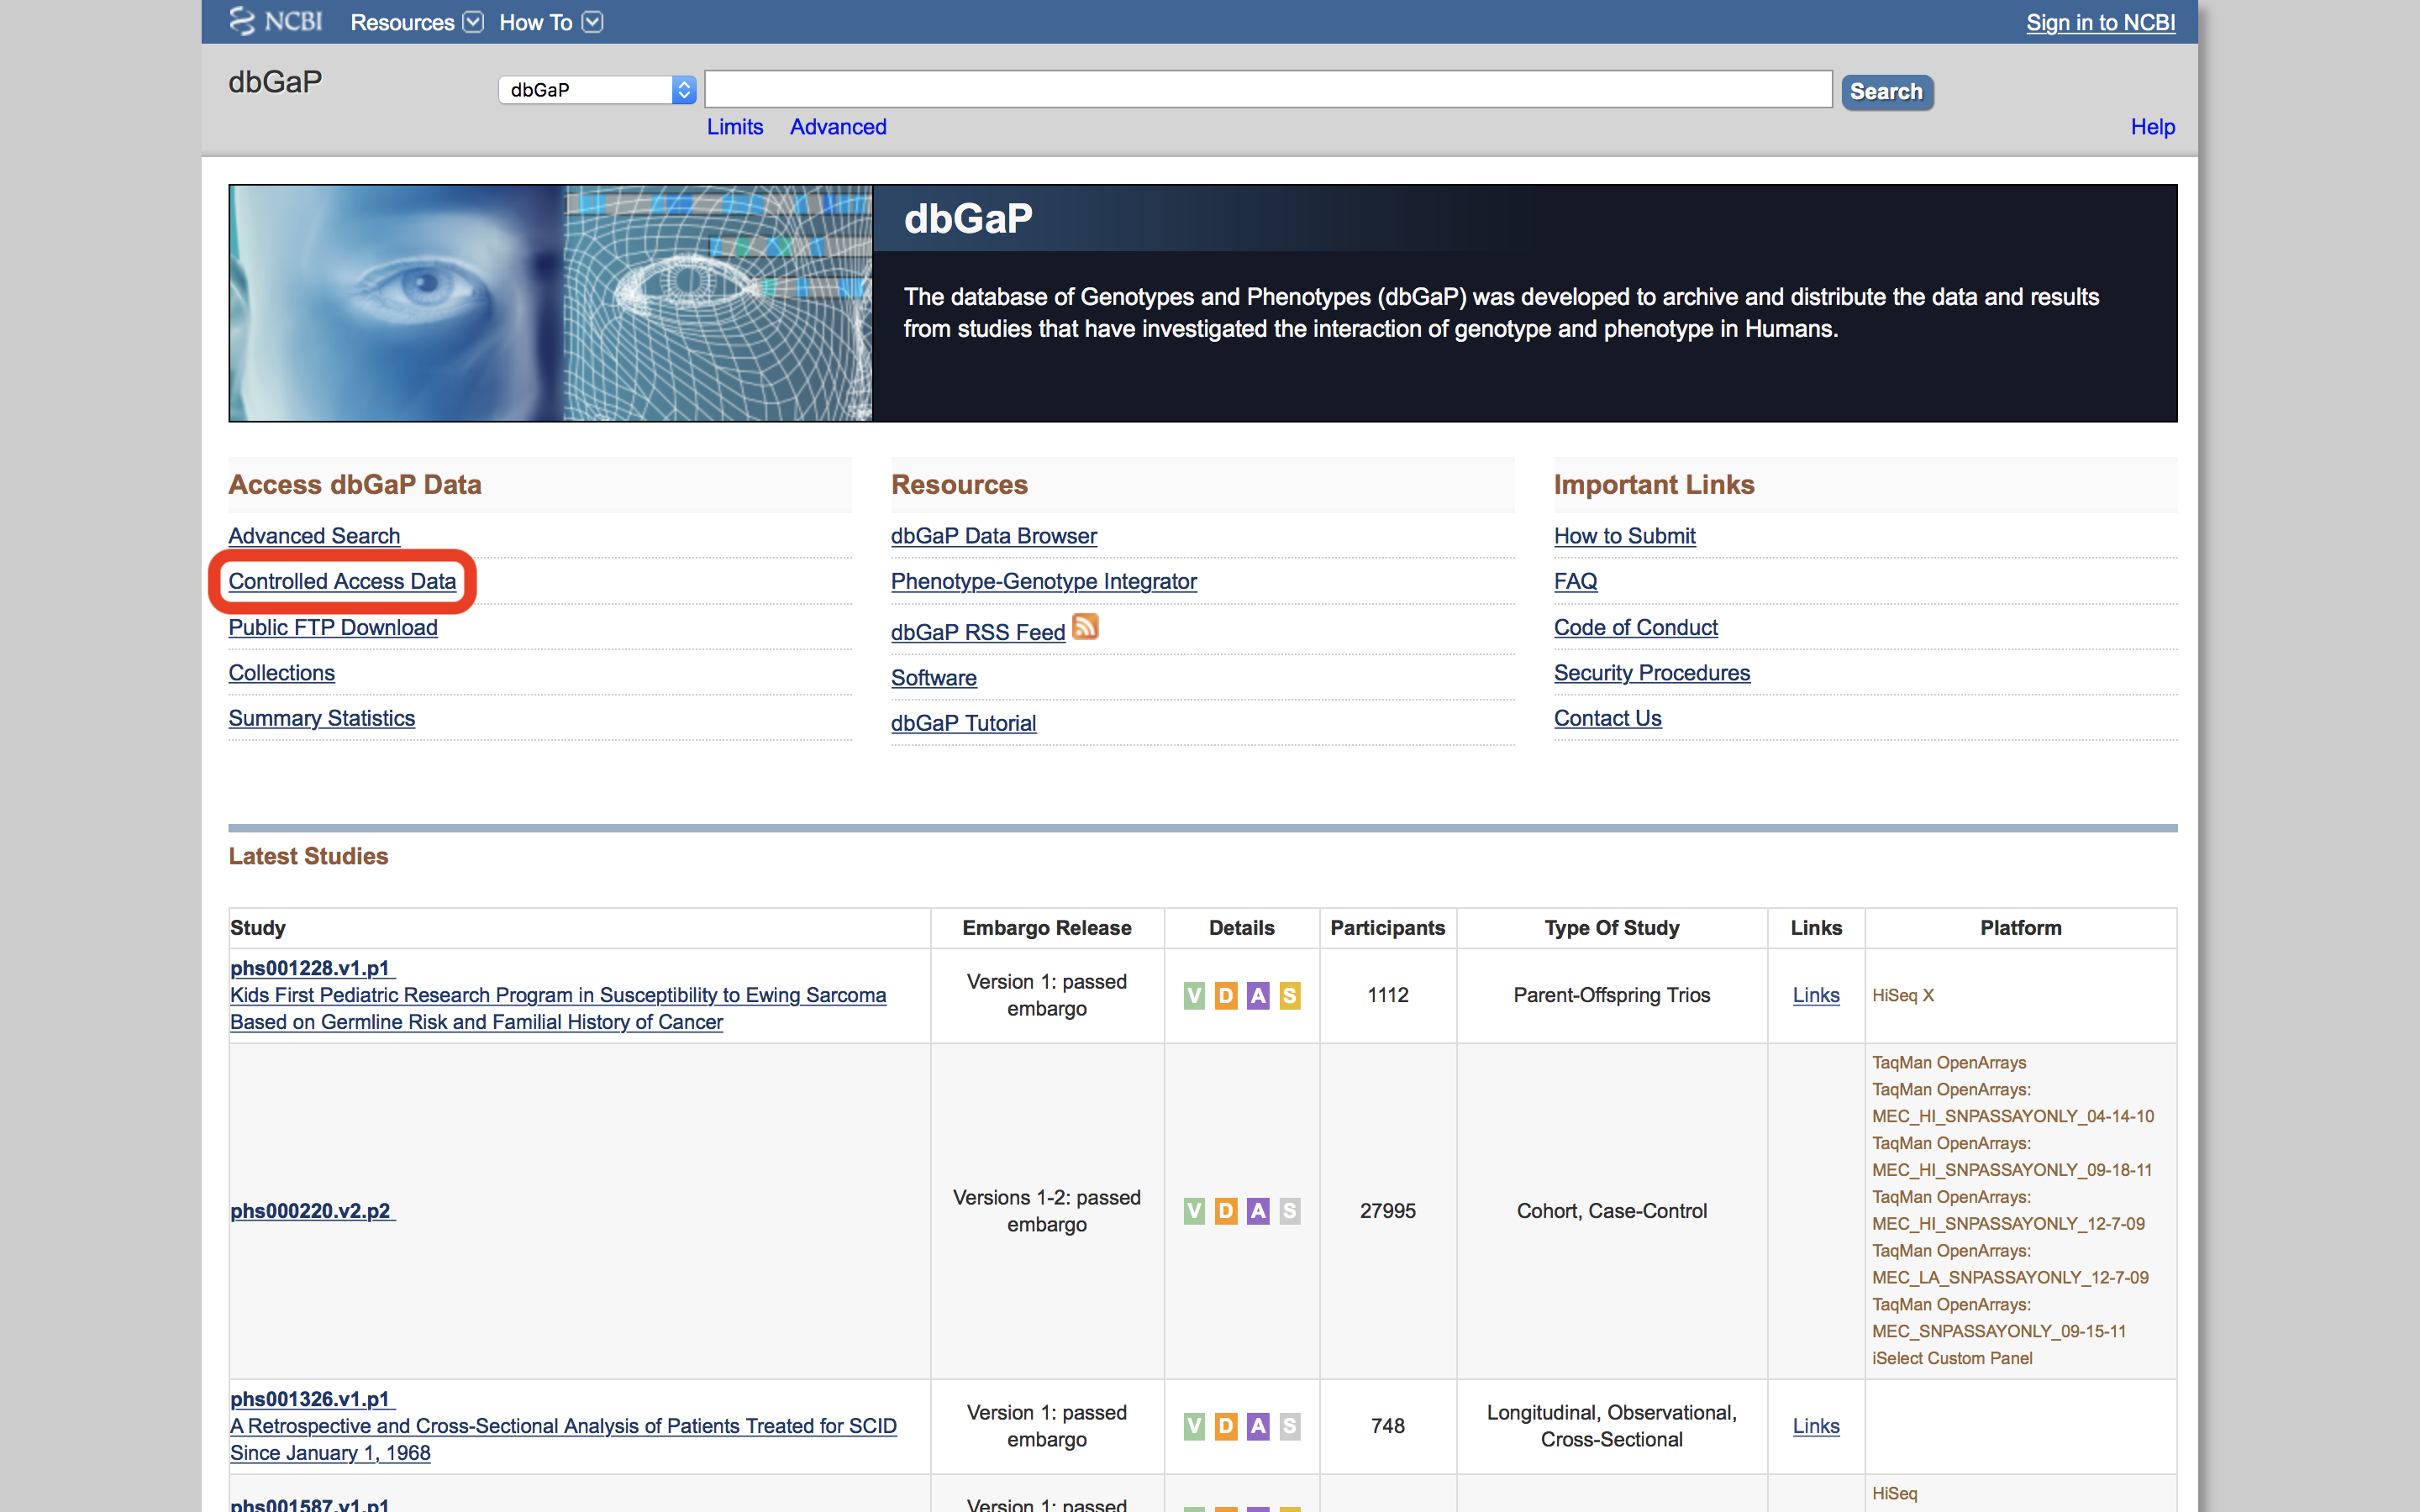
\includegraphics{Screenshots/Screen1.png}

    \hypertarget{b.-click-on-log-in-to-dbgap}{%
\paragraph{b. Click on Log in to dbGaP}\label{b.-click-on-log-in-to-dbgap}}
\ 

    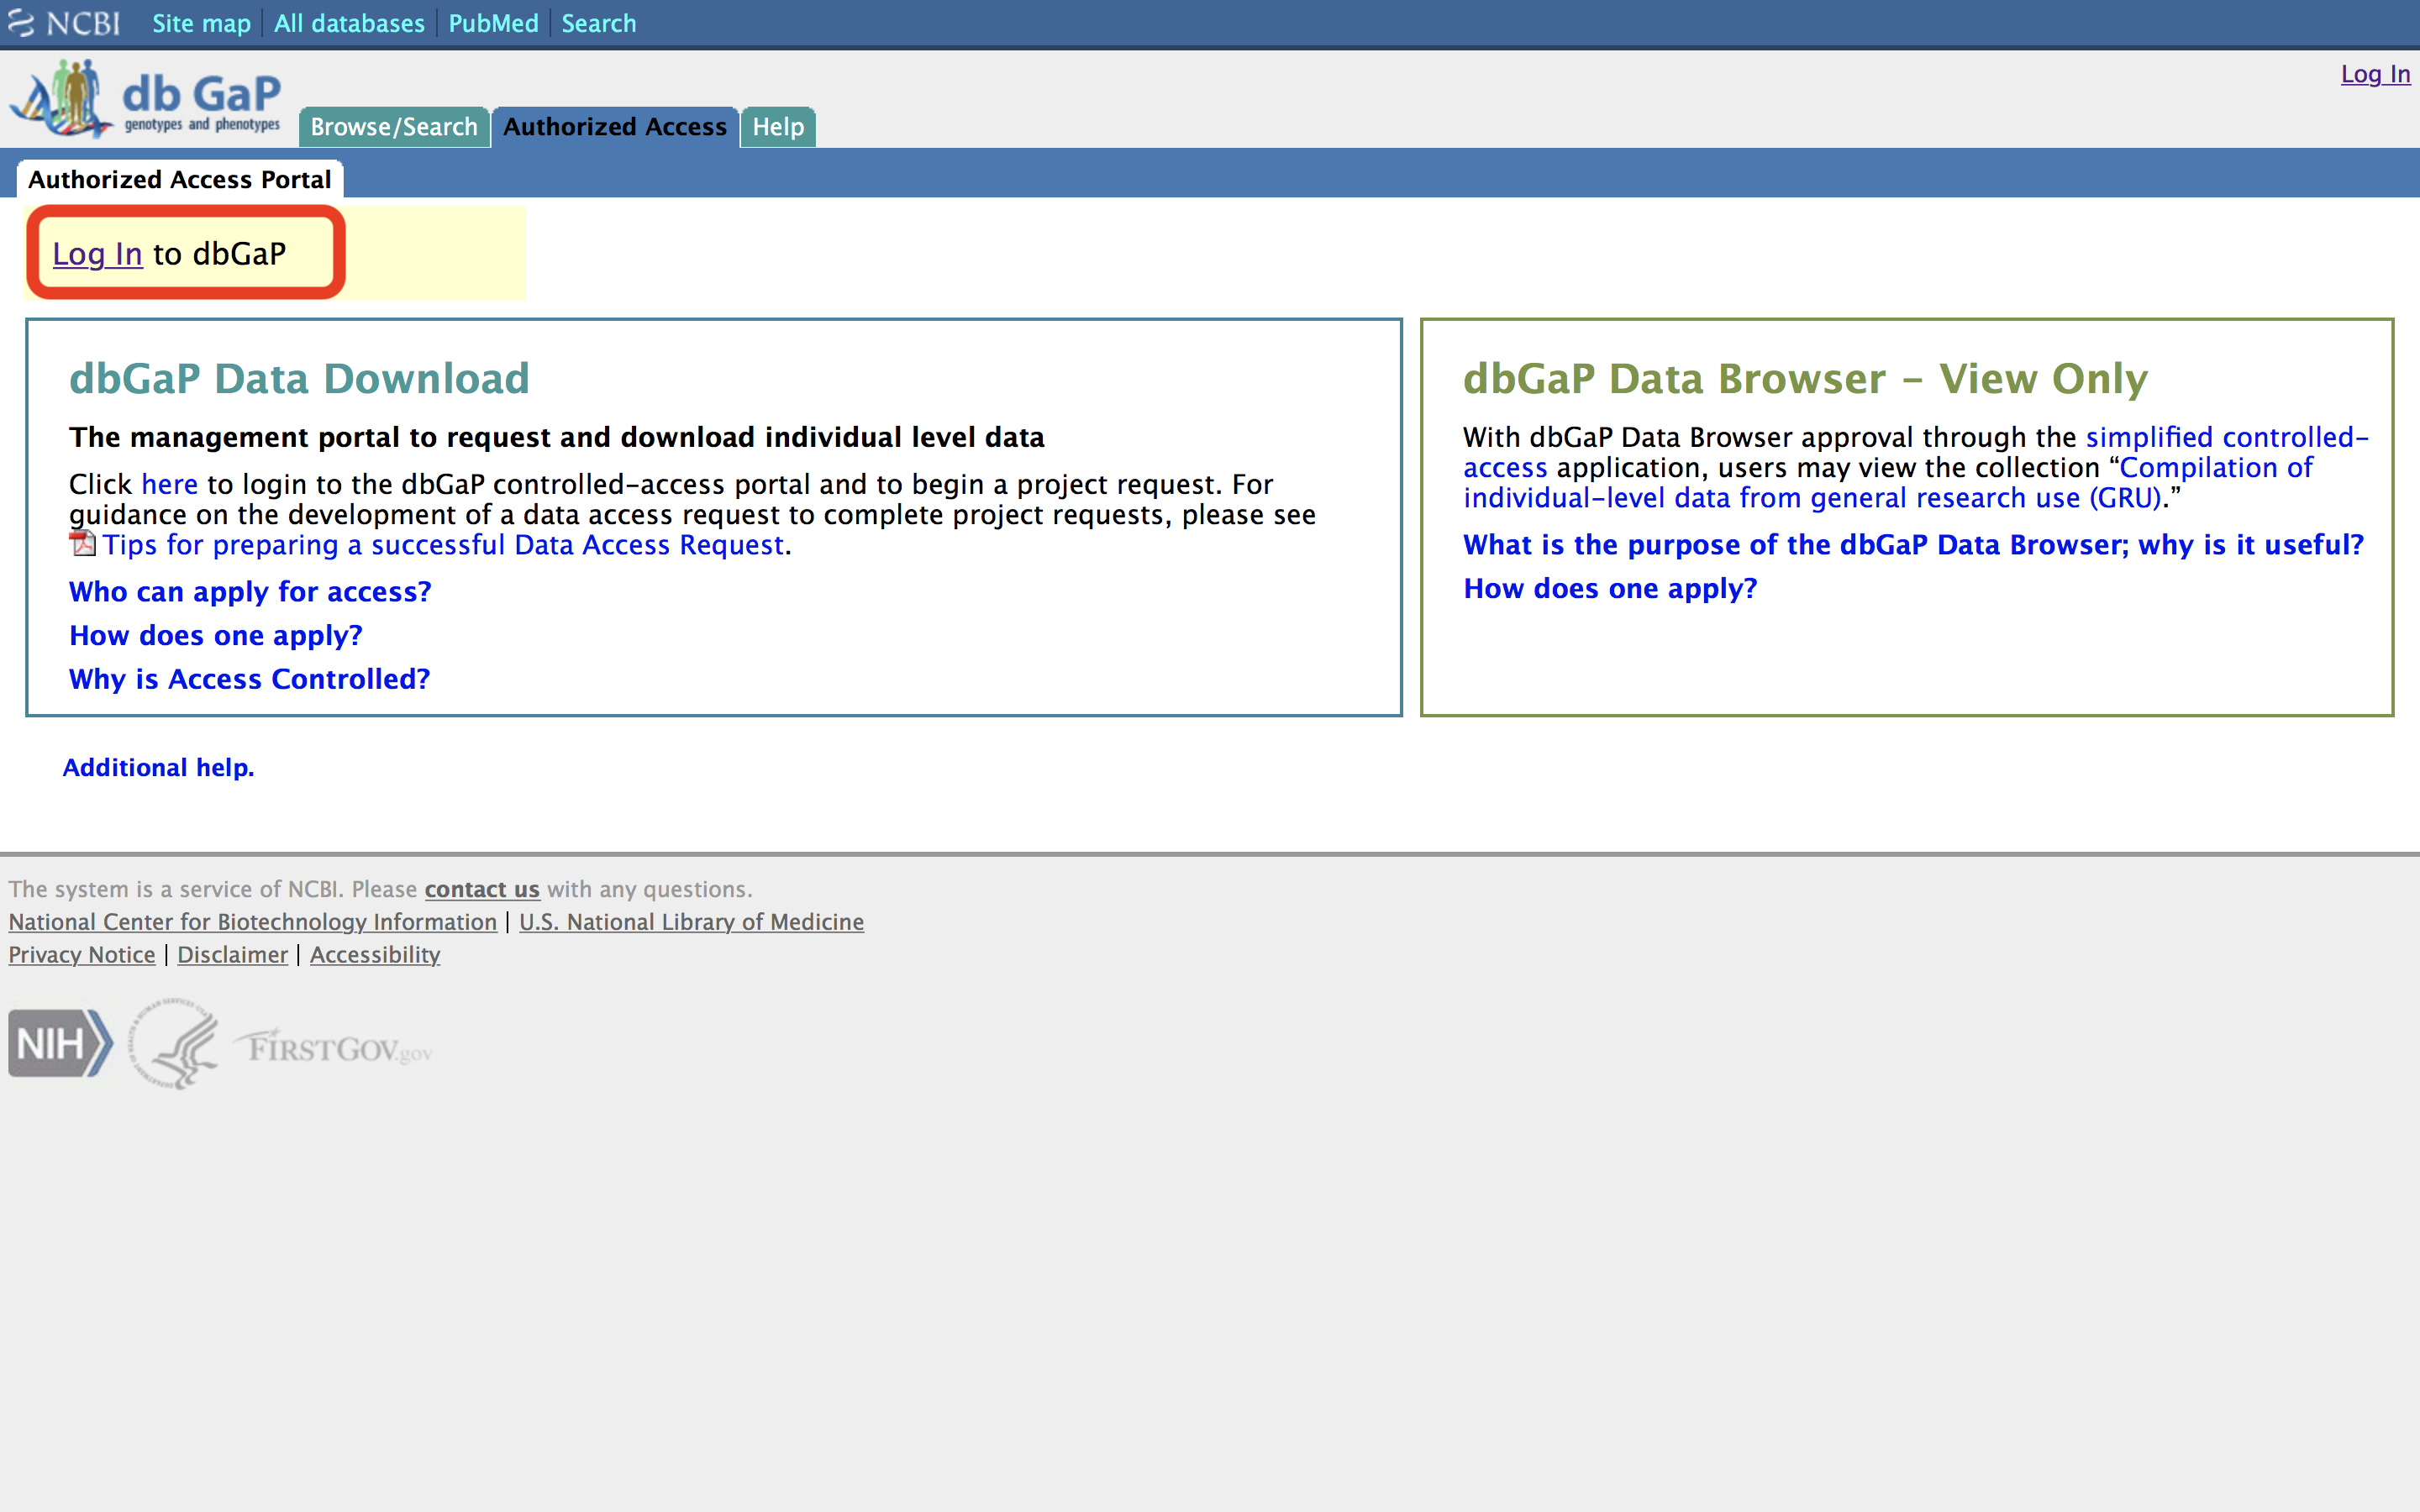
\includegraphics{Screenshots/Screen2.png}

    \hypertarget{c.-identify-yourself-with-your-era-common-id-and-password}{%
\paragraph{c. Identify yourself with your era common ID and password}\label{c.-identify-yourself-with-your-era-common-id-and-password}}
\ 

  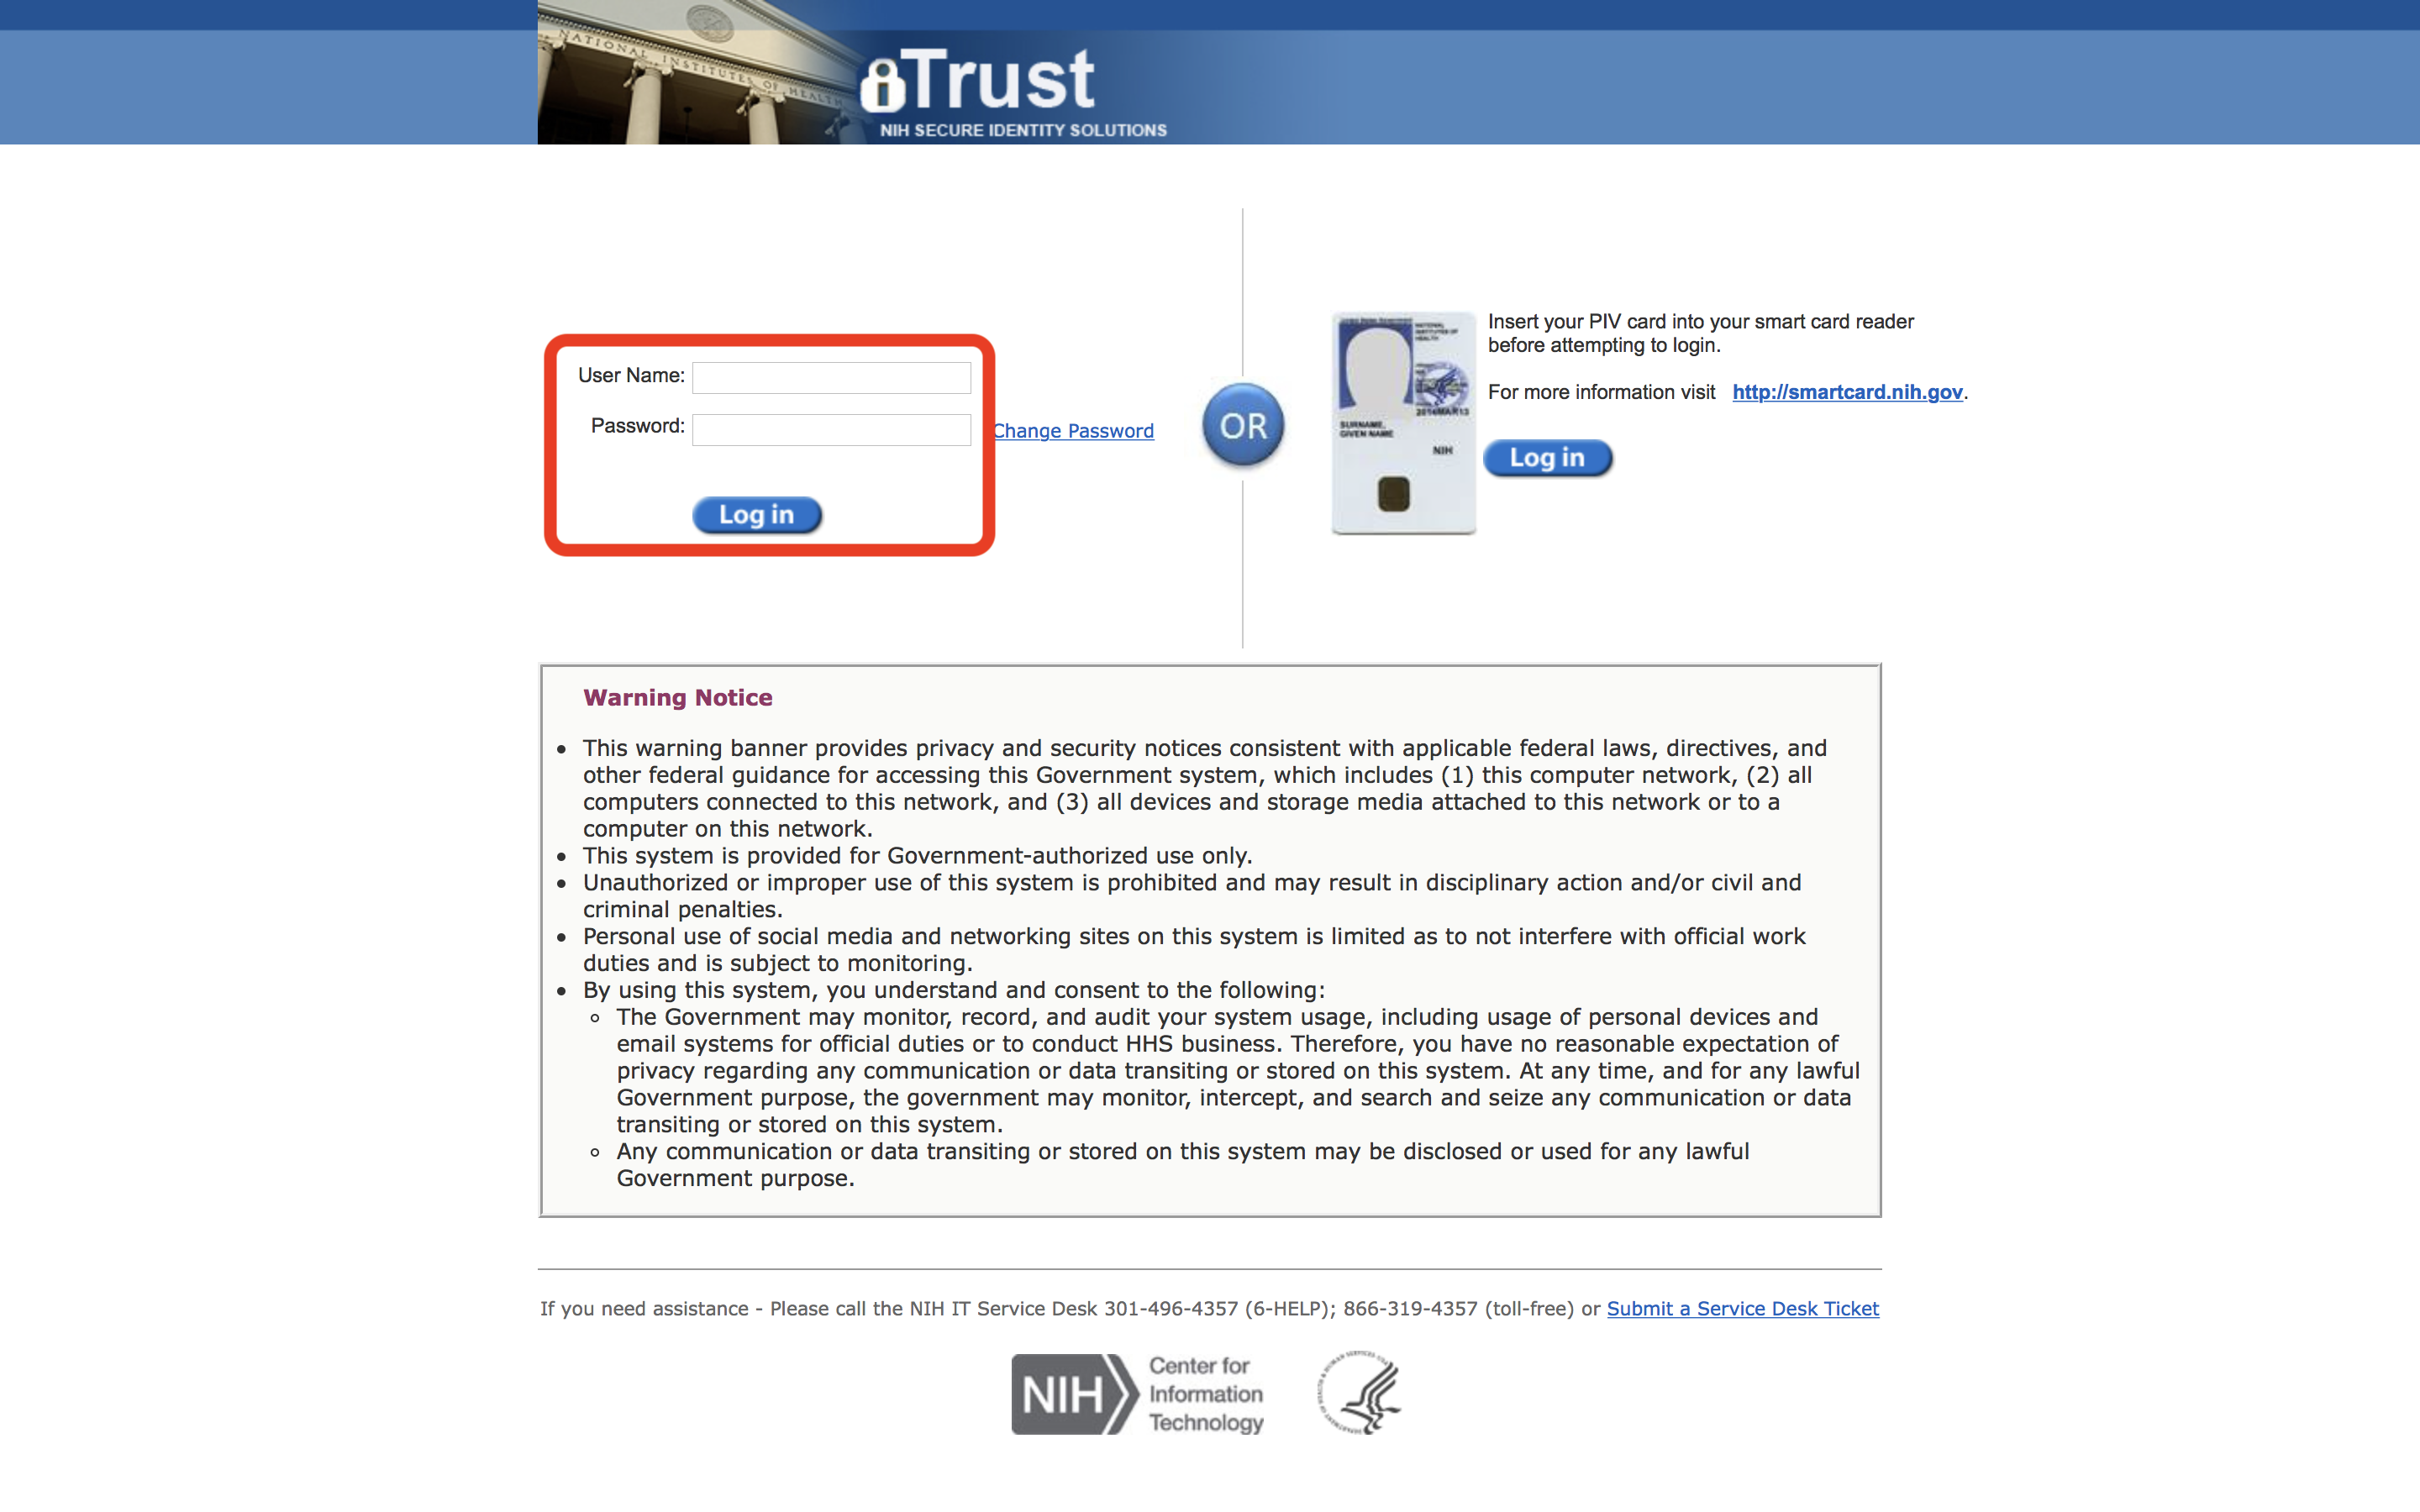
\includegraphics{Screenshots/Screen3.png}

    \hypertarget{d.-get-a-pi-dbgap-repository-key}{%
\paragraph{d. Get a PI dbGaP repository key}\label{d.-get-a-pi-dbgap-repository-key}}
\ 

In order to download the files and to decrypt them, you
will need a decryption key. This key can be found on a PI dbGaP account,
under \texttt{Get\ no\ password\ dbGaP\ repository\ key}

  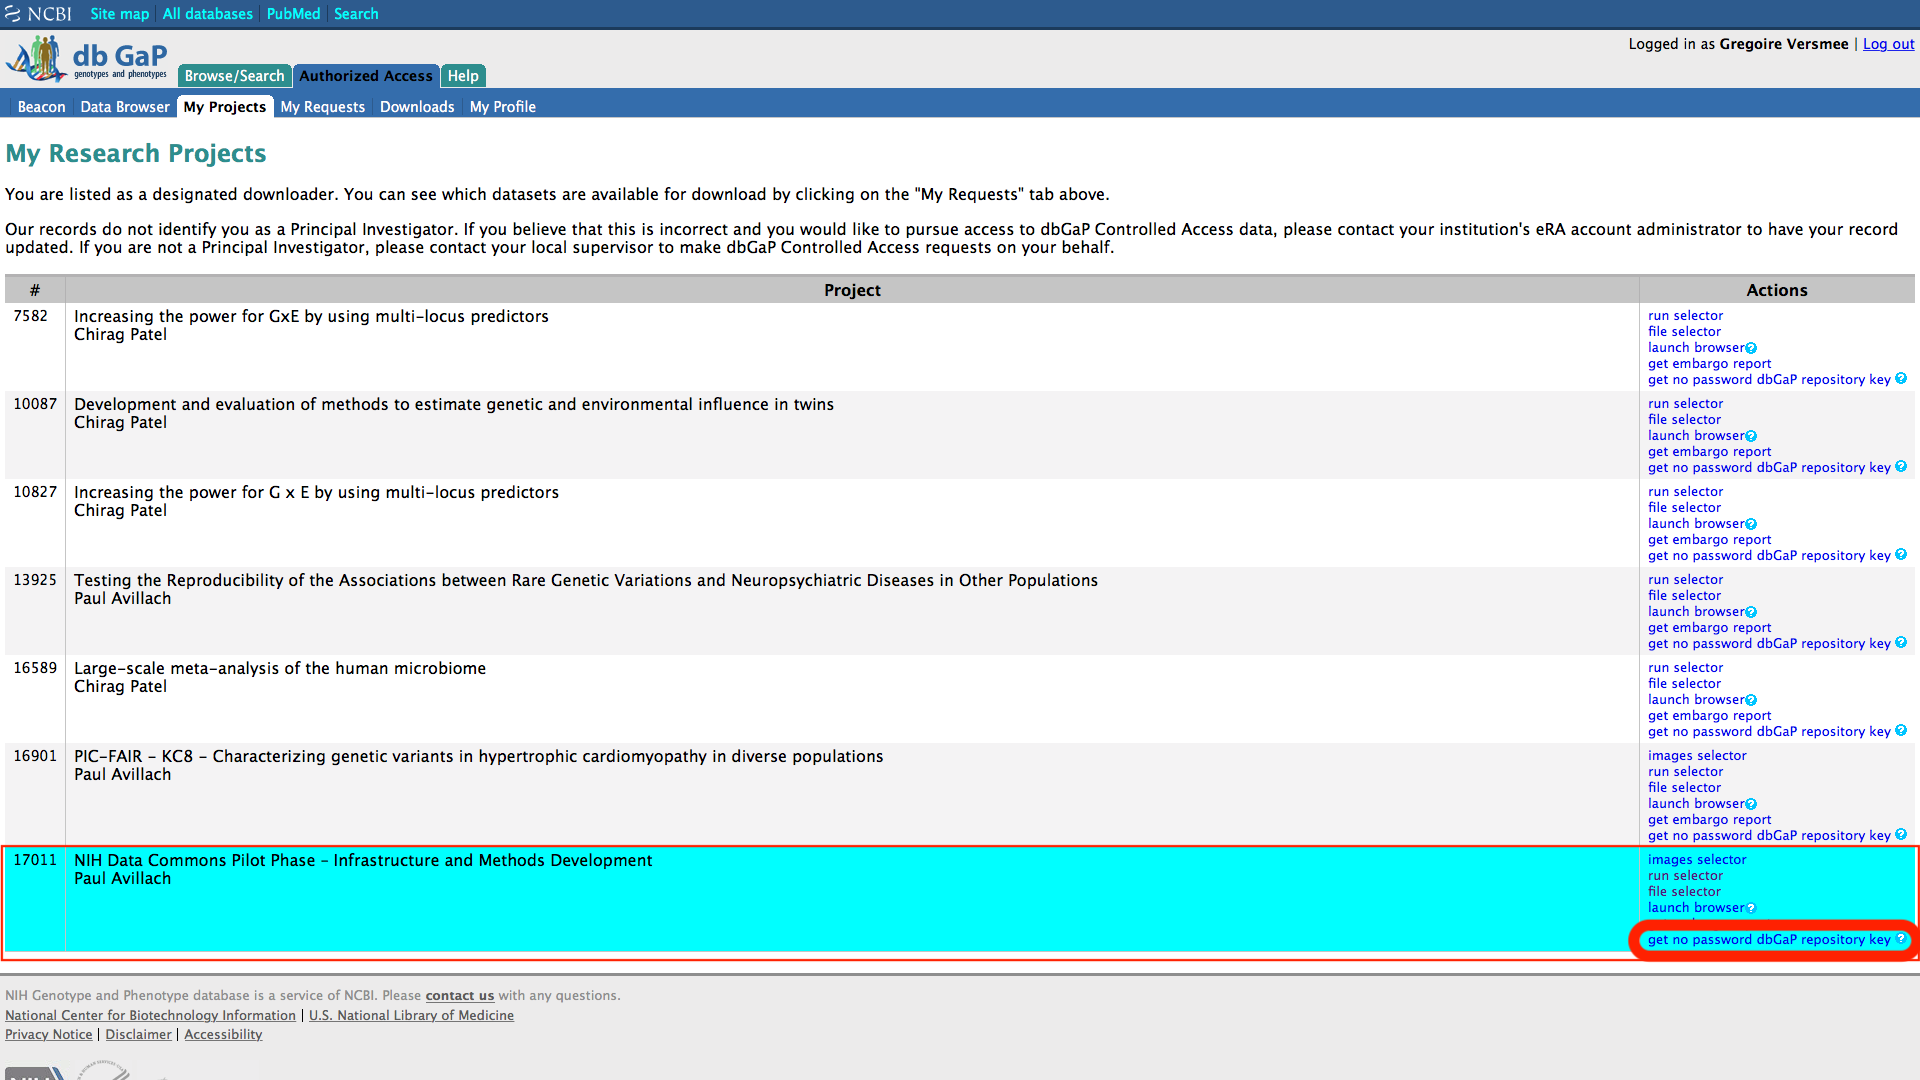
\includegraphics{Screenshots/Screen91.png}

    \hypertarget{decrypt-the-.ncbi_enc-files}{%
\subsubsection{Decrypt the .ncbi\_enc
files}\label{decrypt-the-.ncbi_enc-files}}

On dbGaP, the phenotypic files are encrypted. We created a decryption
function that uses a dockerized version on sratoolkit. To use that
function, you need to have docker installed on your device
(www.docker.com). If you are using the dockerized version of this
software (available at hub.docker.com/r/gversmee/dbgap2x), docker is
already pre-installed, but you'll need to upload your key on the jupyter
working directory. To try the function, we put some pre-encrypted files
on the repo

    \begin{Verbatim}[commandchars=\\\{\}]
{\color{incolor}In [{\color{incolor}15}]:} key \PY{o}{\PYZlt{}\PYZhy{}} \PY{l+s}{\PYZdq{}}\PY{l+s}{prj\PYZus{}17011.ngc\PYZdq{}}
         files \PY{o}{\PYZlt{}\PYZhy{}} \PY{l+s}{\PYZdq{}}\PY{l+s}{encrypted\PYZus{}files\PYZdq{}}
         dbgap.decrypt\PY{p}{(}files\PY{p}{,} key\PY{p}{)}
\end{Verbatim}


    You should see a ``decrypted\_files'' directory in the directory where
your encrypted files are located

    \hypertarget{download-dbgap-files}{%
\subsubsection{3.1. Download dbGaP files}\label{download-dbgap-files}}

\hypertarget{a.-click-on-file-selector}{%
\paragraph{a. Click on ``file
selector''}\label{a.-click-on-file-selector}}
\ 

This gives you access to the dbGaP file selector where you can find all
the files available for the selected project.
\ 

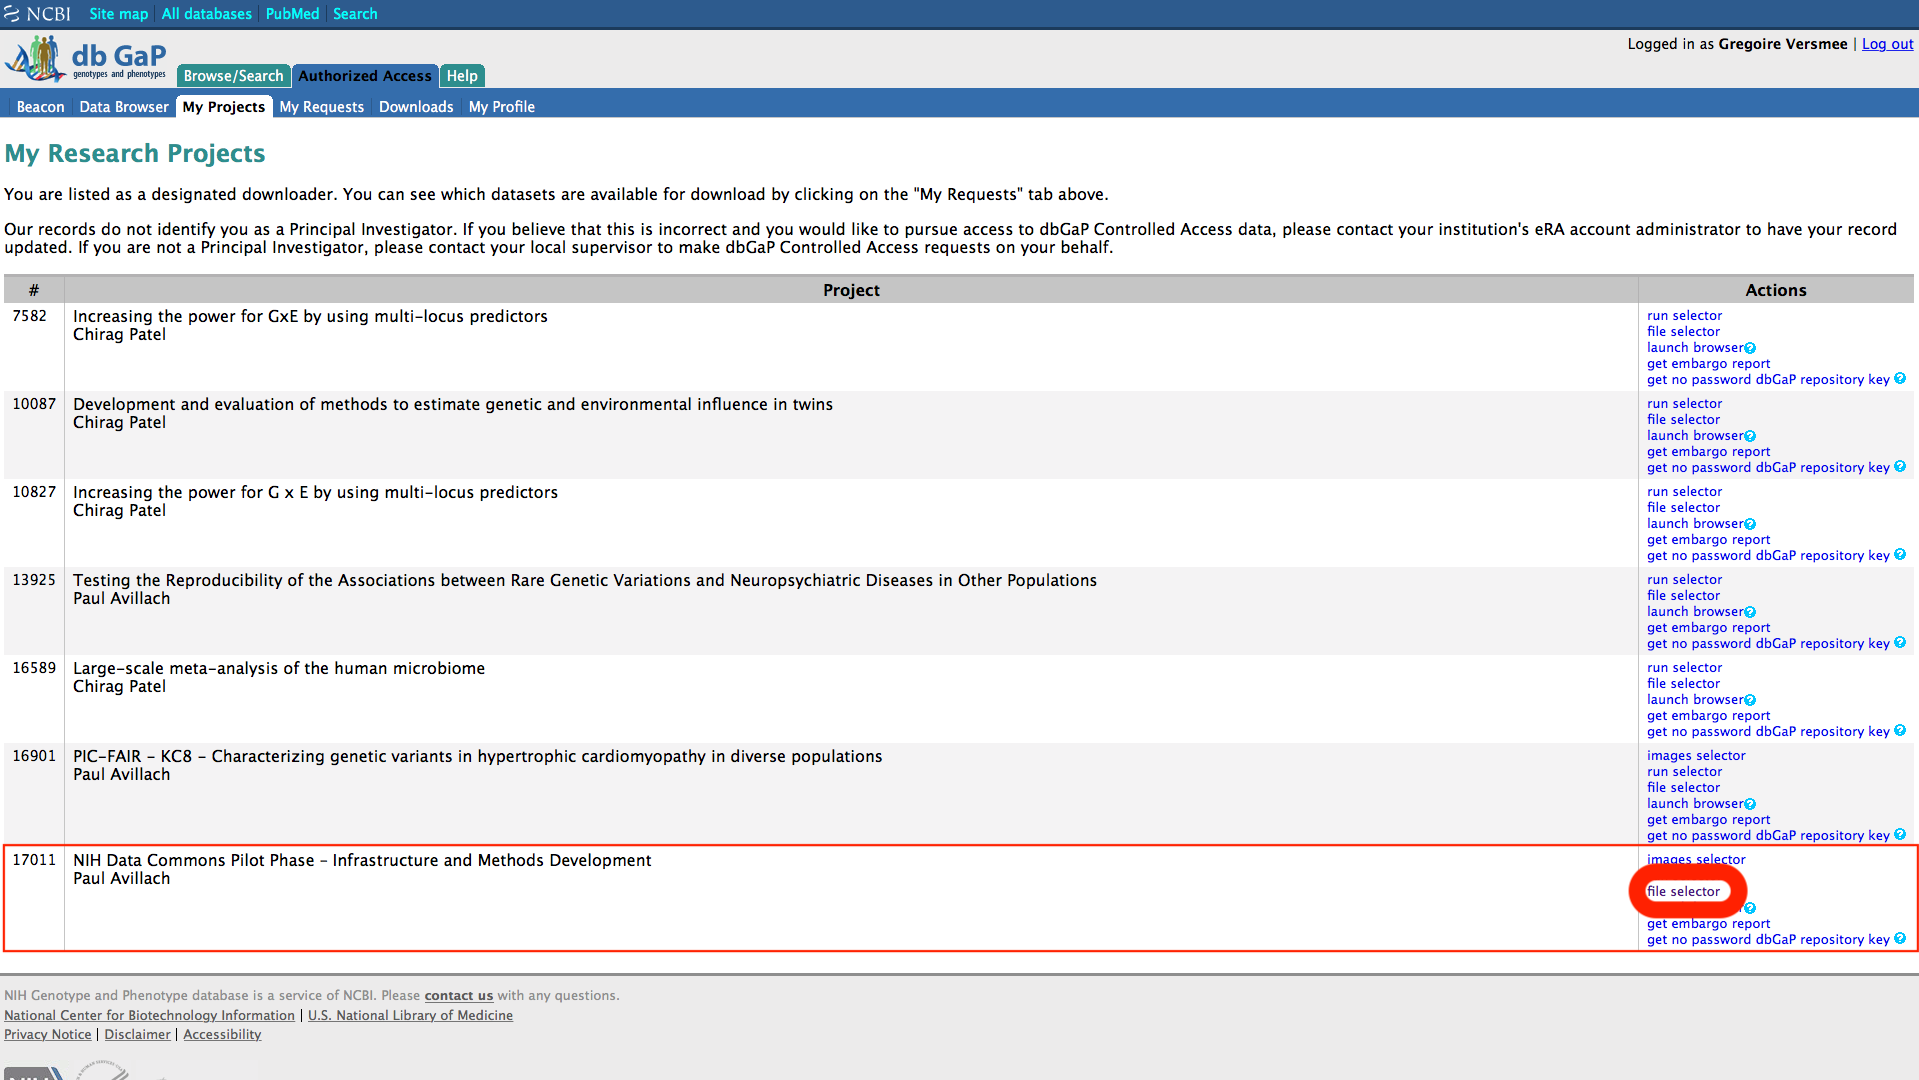
\includegraphics{Screenshots/Screen41.png}
\ 

\hypertarget{b.-filter-by-study-accession}{%
\paragraph{b. Filter by study accession}\label{b.-filter-by-study-accession}}
\ 

Here, we want to get the phenotypic data for the study ``Early
onset COPD'', so after checking \texttt{Study\ accession}, we select
``phs000946''.
\ 

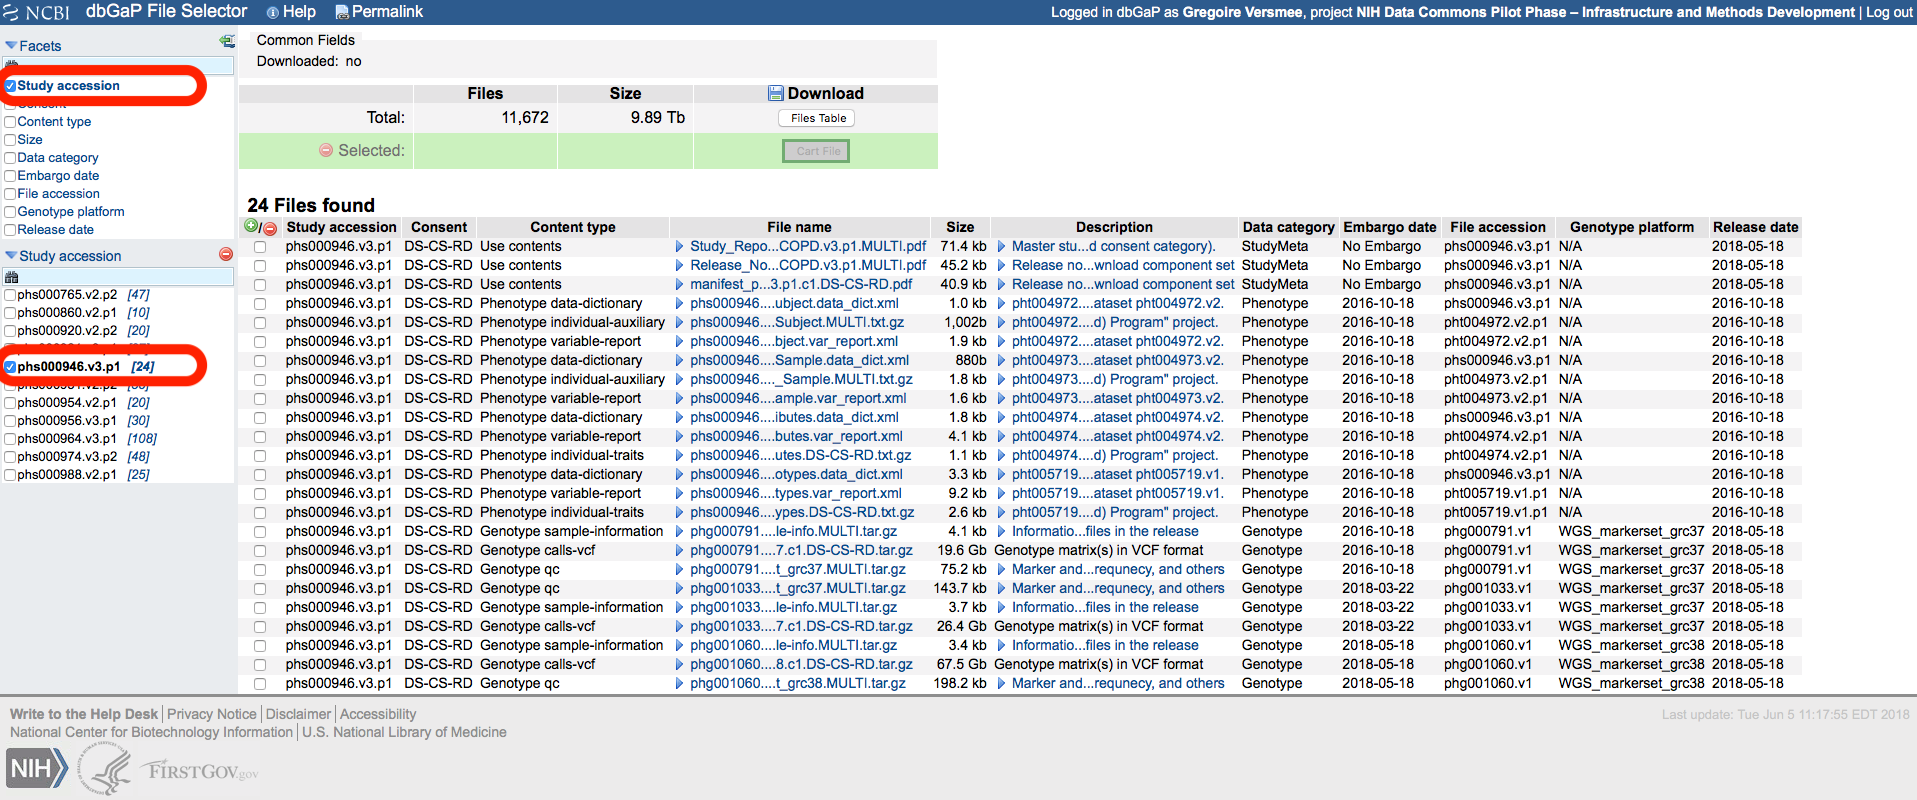
\includegraphics{Screenshots/Screen51.png}

\hypertarget{c-filter-again}{%
\paragraph{c.Filter again}\label{c-filter-again}}
\ 

Since we are only interested in getting the phenotypic
data, let's filter by \texttt{Content\ type} and select
\texttt{phenotype\ individual-auxiliary} and
\texttt{phenotype\ individual-traits}
\ 

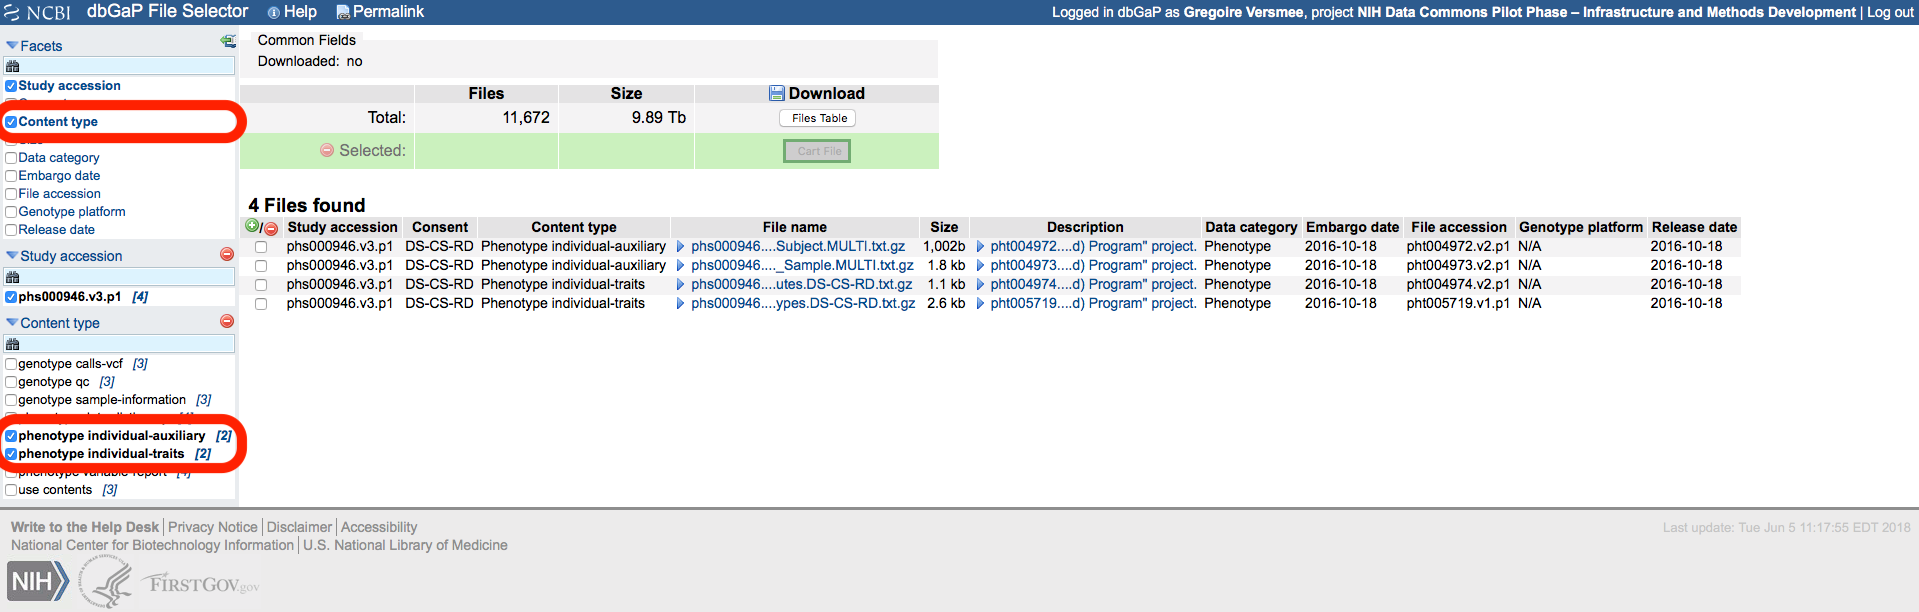
\includegraphics{Screenshots/Screen61.png}
\ 

\hypertarget{d.-select-the-files}{%
\paragraph{d. Select the files}\label{d.-select-the-files}}
\ 

Click on ``+'' to select all the files
\ 

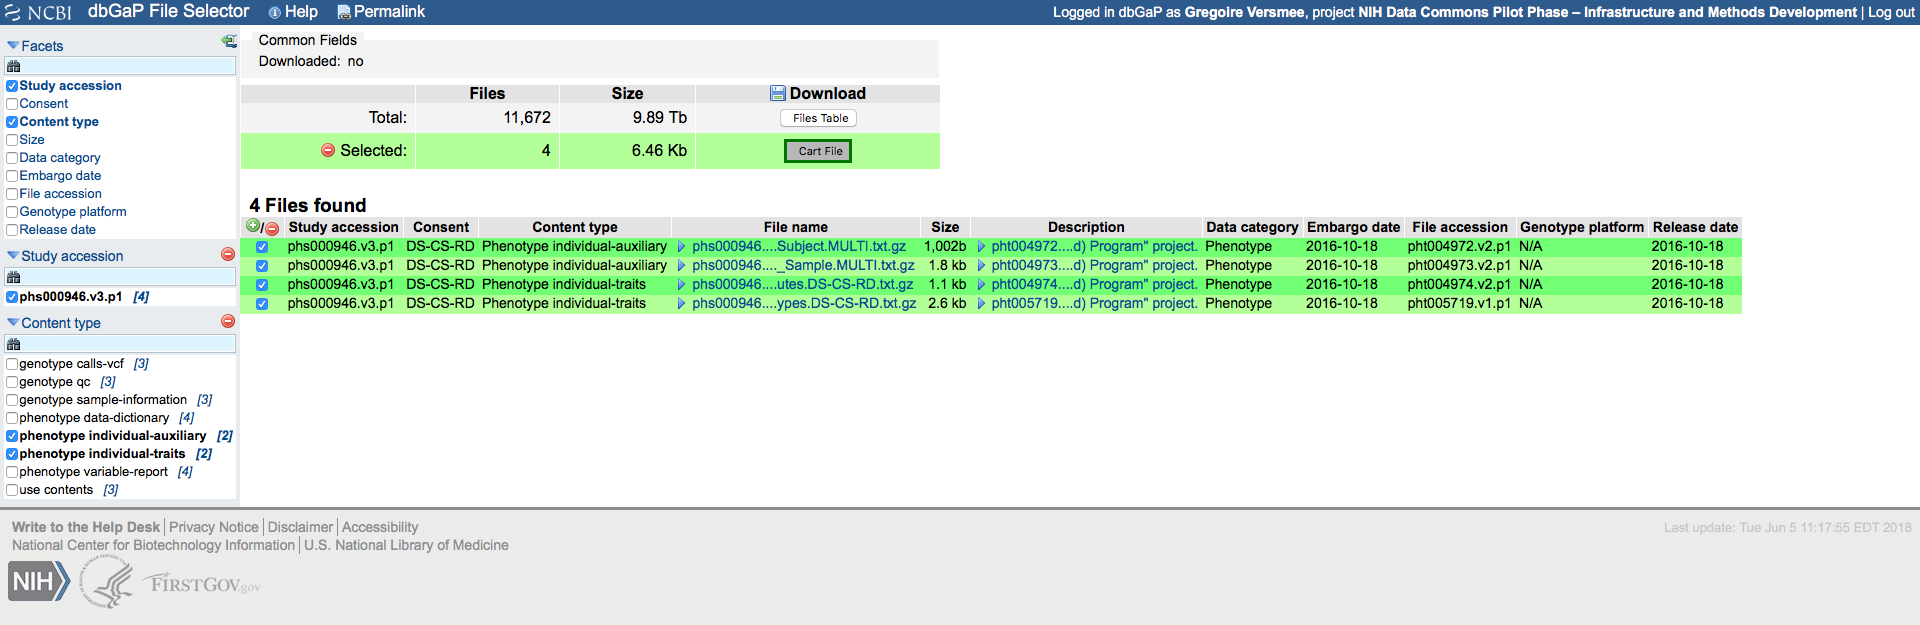
\includegraphics{Screenshots/Screen72.png}
\ 
\hypertarget{e.-click-on-cart-file}{%
\paragraph{e. Click on ``Cart file''}\label{e.-click-on-cart-file}}
\ 

This will downlaod a .krt file in your download folder
\ 

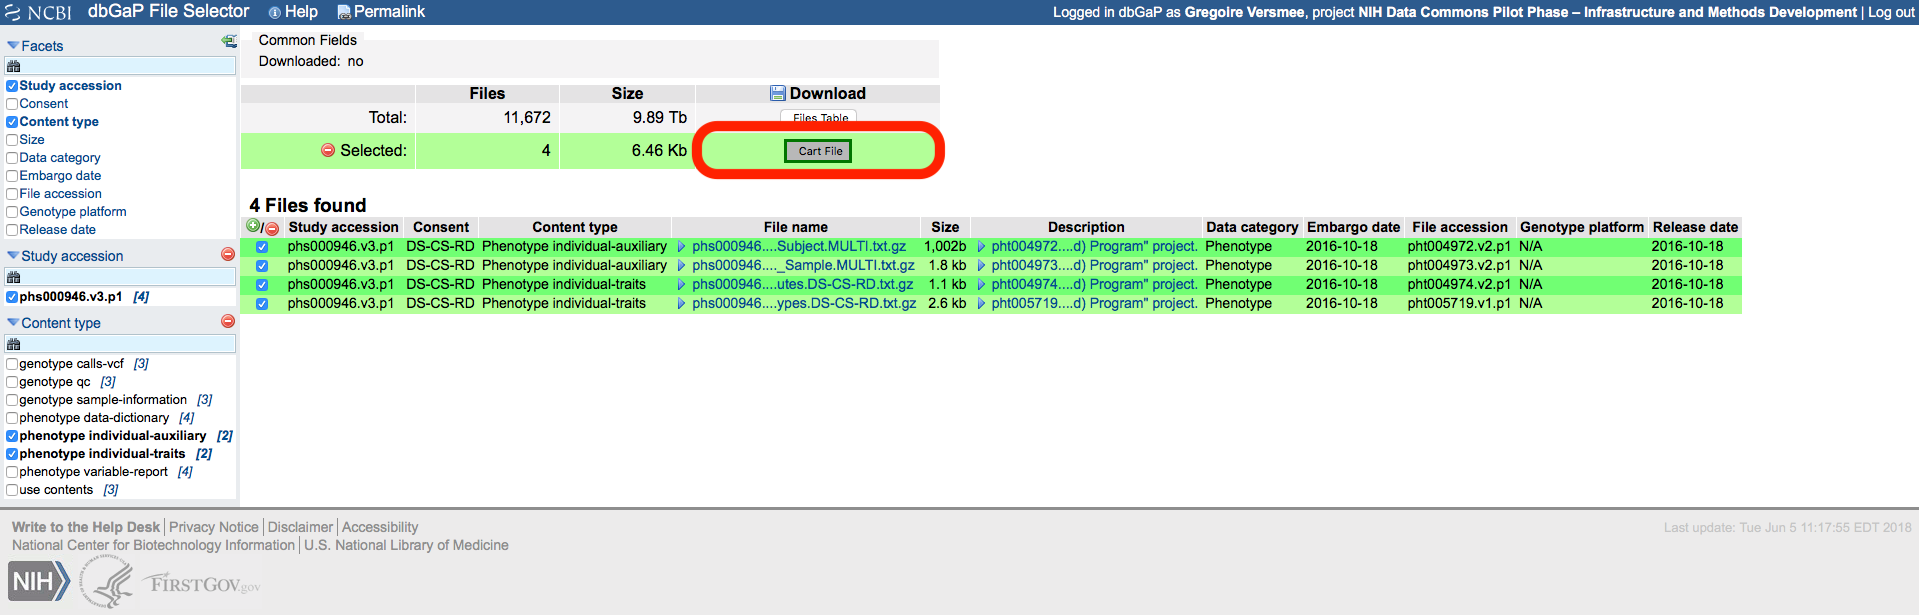
\includegraphics{Screenshots/Screen81.png}
\ 

\hypertarget{f.-download-and-decrypt-the-files-with-a-simple-command}{%
\paragraph{f. Download and decrypt the files with a simple command}\label{f.-download-and-decrypt-the-files-with-a-simple-command}}

    \begin{Verbatim}[commandchars=\\\{\}]
{\color{incolor}In [{\color{incolor}16}]:} key \PY{o}{\PYZlt{}\PYZhy{}} \PY{l+s}{\PYZdq{}}\PY{l+s}{prj\PYZus{}17011.ngc\PYZdq{}}
         cart \PY{o}{\PYZlt{}\PYZhy{}} \PY{l+s}{\PYZdq{}}\PY{l+s}{cart\PYZus{}prj17011\PYZus{}201810151143.krt\PYZdq{}}
         dbgap.download\PY{p}{(}cart\PY{p}{,} key\PY{p}{)}
\end{Verbatim}


    You should see in your working directory a new one name dbGaP-*** that
contains your files


    % Add a bibliography block to the postdoc
    
    
    
    \end{document}
